%===============================================================================
% LaTeX sjabloon voor de bachelorproef toegepaste informatica aan HOGENT
% Meer info op https://github.com/HoGentTIN/latex-hogent-report
%===============================================================================

\documentclass[dutch,dit,thesis]{hogentreport}

% TODO:
% - If necessary, replace the option `dit`' with your own department!
%   Valid entries are dbo, dbt, dgz, dit, dlo, dog, dsa, soa
% - If you write your thesis in English (remark: only possible after getting
%   explicit approval!), remove the option "dutch," or replace with "english".

\usepackage{lipsum} % For blind text, can be removed after adding actual content

%% Pictures to include in the text can be put in the graphics/ folder
\graphicspath{{../graphics/}}

%% For source code highlighting, requires pygments to be installed
%% Compile with the -shell-escape flag!
% \usepackage[chapter]{minted}
%% If you compile with the make_thesis.{bat,sh} script, use the following
%% import instead:
\usepackage[chapter,outputdir=../output]{minted}
\usemintedstyle{solarized-light}

%% Formatting for minted environments.
\setminted{%
    autogobble,
    frame=lines,
    breaklines,
    linenos,
    tabsize=4
}

%% Ensure the list of listings is in the table of contents
\renewcommand\listoflistingscaption{%
    \IfLanguageName{dutch}{Lijst van codefragmenten}{List of listings}
}
\renewcommand\listingscaption{%
    \IfLanguageName{dutch}{Codefragment}{Listing}
}
\renewcommand*\listoflistings{%
    \cleardoublepage\phantomsection\addcontentsline{toc}{chapter}{\listoflistingscaption}%
    \listof{listing}{\listoflistingscaption}%
}

% Other packages not already included can be imported here

%%---------- Document metadata -------------------------------------------------
% Replaced this with your own information
\author{Maarten Adriaenssens}
\supervisor{Mevr. L. De Mol}
\cosupervisor{Dhr. T. Cuelenaere en Dhr. J. Buysse}
\title[Optionele ondertitel]%
    {Integratie en vervanging van DECT-systemen met 5G-technologie voor zorgsimulaties binnen HOGENT}
\academicyear{\advance\year by -1 \the\year--\advance\year by 1 \the\year}
\examperiod{1}
\degreesought{\IfLanguageName{dutch}{Professionele bachelor in de toegepaste informatica}{Bachelor of applied computer science}}
\partialthesis{false} %% To display 'in partial fulfilment'
%\institution{Internshipcompany BVBA.}

%% Add global exceptions to the hyphenation here
\hyphenation{back-slash}

%% The bibliography (style and settings are  found in hogentthesis.cls)
\addbibresource{bachproef.bib}            %% Bibliography file
\addbibresource{../voorstel/voorstel.bib} %% Bibliography research proposal
\defbibheading{bibempty}{}

%% Prevent empty pages for right-handed chapter starts in twoside mode
\renewcommand{\cleardoublepage}{\clearpage}

\renewcommand{\arraystretch}{1.2}

%% Content starts here.
\begin{document}

%---------- Front matter -------------------------------------------------------

\frontmatter

\hypersetup{pageanchor=false} %% Disable page numbering references
%% Render a Dutch outer title page if the main language is English
\IfLanguageName{english}{%
    %% If necessary, information can be changed here
    \degreesought{Professionele Bachelor toegepaste informatica}%
    \begin{otherlanguage}{dutch}%
        \maketitle%
    \end{otherlanguage}%
}{}

%% Generates title page content
\maketitle
\hypersetup{pageanchor=true}

%%=============================================================================
%% Voorwoord
%%=============================================================================

\chapter*{\IfLanguageName{dutch}{Woord vooraf}{Preface}}%
\label{ch:voorwoord}

% Alarmen mag je zeker niet negeren, zeker niet als je moe bent. 

% Door mijn studies heen heb ik altijd een praktische kijk gehad op andere sectoren. Vaak met het idee, kunnen we dit niet verbeteren met nieuwe technologieën. Dus toen ik de kans kreeg om een bachelorproef te schrijven over een onderwerp dat nieuwe technologie te gebruiken om een maatschappelijke impact te hebben, was ik meteen enthousiast.

% Het doel van deze bachelorproef is om het zorgverlenend personeel te ondersteunen met een nieuw communicatie systeem dat de stress bij zorgverleners vermindert en hierdoor hun focus en aandacht verbeterd, met een betere patiëntenzorg en efficiëntere ziekenhuiswerking tot gevolg.

% Dit onderzoek biedt me de kans om mijn kennis mijn theoretische kennis in netwerken te verdiepen in het mobiele netwerk aspect. Het is de synergie tussen de zorg en de technologie die mij aanspreekt. Het idee dat de bachelorproef een directe impact kan hebben op de zorgopleiding en zorgsector is een extra motivatie. 

% Deze bachelorproef maakt deel uit van het 5Genius project. Dit is een samenwerkingsproject tussen HOGENT en CityMesh, met steun van Europese Unie. Beide partijen hebben mij ondersteund op hun eigen manier. HOGENT heeft het 360° Zorglab naar voor geschoven als niet-technische ondersteuning. 360° Zorglab was voor mij als IT-student een raam, langswaar ik naar de werking en het gebeuren binnen een (gesimuleerde) zorgomgeving kon gadeslaan. CityMesh heeft mij technische ondersteuning geboden als partner in het 5Genius project. Zij hebben, in hun samenwerking met HOGENT, mij hardware en de kennis, die nodig was om dit project tot een goed einde te brengen, aangerijkt.

% Ik wens specifiek mij co-promotoren, Dhr. T. Cuelenaere, Dhr. J. Buysse en Dhr. M. De Dekoninck, te bedanken voor hun begeleiding en ondersteuning. Hun kritische feedback en constructieve bijdragen hebben een belangrijke rol gespeeld in de totstandkoming van dit onderzoek. Mijn promotor Mevr. L. De Mol, voor haar begeleiding, geduld en overzicht dat zij geboden heeft die ik soms miste.
% Mijn ouders en zus als spellingscontrole en testpubliek. Ik denk dat zij intussen ook het 5G systeem goed kennen.

Alarmen mag je zeker niet negeren, zeker niet als je moe bent. Hoe kan je nu IT inzetten om stress bij zorgverleners te verminderen? Dat is wat deze bachelorproef probeert te beantwoorden.
\\
Door mijn studies heen heb ik altijd een praktische kijk gehad op andere sectoren. Vaak met de insteek: kunnen we dit niet verbeteren met nieuwe technologieën? Dus toen ik de kans kreeg om een bachelorproef te schrijven over een onderwerp dat nieuwe technologie gebruikt om een maatschappelijke impact te hebben, was ik meteen enthousiast.
\\\\
Het doel van deze bachelorproef is om het zorgverlenend personeel te ondersteunen met een nieuw communicatiesysteem dat de stress vermindert en hierdoor hun focus en aandacht verbetert, met een betere patiëntenzorg en efficiëntere ziekenhuiswerking tot gevolg.
\\
Dit onderzoek biedt me de kans om mijn theoretische kennis van netwerken te verdiepen in het mobiele netwerk aspect. Het is de synergie tussen de zorg en de technologie die mij aanspreekt. Het idee dat de bachelorproef een directe impact kan hebben op de zorgopleiding en zorgsector is een extra motivatie.
\\\\
Deze bachelorproef maakt deel uit van het 5Genius project. Dit is een samenwerkingsproject tussen HOGENT en CityMesh, met steun van de Europese Unie. Beide partijen hebben mij ondersteund op hun eigen manier. HOGENT heeft het 360° Zorglab naar voren geschoven als niet-technische ondersteuning. 360° Zorglab was voor mij als IT-student een raam, waarlangs ik de werking en het gebeuren binnen een (gesimuleerde) zorgomgeving kon gadeslaan. CityMesh heeft mij technische ondersteuning geboden als partner in het 5Genius project. Zij hebben, in hun samenwerking met HOGENT, mij hardware en kennis, die nodig was om dit project tot een goed einde te brengen, aangereikt.
\\\\
Ik wens specifiek mijn co-promotoren, Dhr. T. Cuelenaere, Dhr. J. Buysse en Dhr. M. De Dekoninck, te bedanken voor hun begeleiding en ondersteuning. Hun kritische feedback en constructieve bijdragen hebben een belangrijke rol gespeeld in de totstandkoming van dit onderzoek. Mijn promotor Mevr. L. De Mol, voor haar begeleiding, geduld en overzicht dat zij geboden heeft die ik soms miste.
Mijn ouders en zus als spellingscontrole en testpubliek. Ik denk dat zij intussen ook het 5G-systeem goed kennen.

%% TODO:
%% Het voorwoord is het enige deel van de bachelorproef waar je vanuit je
%% eigen standpunt (``ik-vorm'') mag schrijven. Je kan hier bv. motiveren
%% waarom jij het onderwerp wil bespreken.
%% Vergeet ook niet te bedanken wie je geholpen/gesteund/... heeft

%%=============================================================================
%% Samenvatting
%%=============================================================================

% TODO: De "abstract" of samenvatting is een kernachtige (~ 1 blz. voor een
% thesis) synthese van het document.
%
% Een goede abstract biedt een kernachtig antwoord op volgende vragen:
%
% 1. Waarover gaat de bachelorproef?
% 2. Waarom heb je er over geschreven?
% 3. Hoe heb je het onderzoek uitgevoerd?
% 4. Wat waren de resultaten? Wat blijkt uit je onderzoek?
% 5. Wat betekenen je resultaten? Wat is de relevantie voor het werkveld?
%
% Daarom bestaat een abstract uit volgende componenten:
%
% - inleiding + kaderen thema
% - probleemstelling
% - (centrale) onderzoeksvraag
% - onderzoeksdoelstelling
% - methodologie
% - resultaten (beperk tot de belangrijkste, relevant voor de onderzoeksvraag)
% - conclusies, aanbevelingen, beperkingen
%
% LET OP! Een samenvatting is GEEN voorwoord!

%%---------- Nederlandse samenvatting -----------------------------------------
%
% TODO: Als je je bachelorproef in het Engels schrijft, moet je eerst een
% Nederlandse samenvatting invoegen. Haal daarvoor onderstaande code uit
% commentaar.
% Wie zijn bachelorproef in het Nederlands schrijft, kan dit negeren, de inhoud
% wordt niet in het document ingevoegd.

% \IfLanguageName{english}{%
% \selectlanguage{dutch}
% \chapter*{Samenvatting}
% \lipsum[1-4]
% \selectlanguage{english}
% }{}

%%---------- Samenvatting -----------------------------------------------------
% De samenvatting in de hoofdtaal van het document

\chapter*{\IfLanguageName{dutch}{Samenvatting}{Abstract}}

Communicatie is een heel belangrijk onderdeel van een goede werking van een ziekenhuis. Toch is het meest gebruikte communicatie systeem in ziekehuizen sinds 1993 niet veranderd van principe. Dit pricipe/systeem is het \gls{dect}-systeem. Dit onderzoek focust zich op het onderzoeken van de mogelijke technologieën die kunnen worden ingezet ingezet om de communicatie aan te pakken in de gezondheidszorg. De reden van dit onderzoek is om een kwaliteitsvol alternatief te bieden voor de vervanging van het \gls{dect}-systeem. Een reden voor deze vervanging is dat deze aanleiding geeft tot alarmmoeheid.
Volgens \textcite{Ferrara2023} kan alarmmoeheid worden omschreven als ''een overprikkeling of zintuiglijke overbelasting, in staat tot het veroorzaken van gevoelloosheid ten opzichte van alarmen door een te groot aantal alarmen die foutief of klinisch onbelangrijk zijn.''.\\ Eerst zal er breed worden gekeken naar alle mogelijke innovaties, nadien wordt er gefocust op een toepassing van een privaat 5G-netwerk. 
Vervolgens worden er twee  (\gls{poc}) gemaakt. De eerste is een testomgeving, lokaal op de laptop van de student. De tweede \gls{poc} is een praktische realisatie; deze wordt ontwikkeld op kleine schaal, maar met uitbreidingsmogelijkheden. Tenslotte wordt er ook onderzocht wat de kost is van een 5G-deployment. Dit wordt verwerkt zodat er een overzicht is van wanneer een ziekenhuis het zou overwegen om de kosten te kunnen verantwoorden.\\
Er wordt verwacht dat de \gls{poc}'s beiden worden gerealiseerd en een overzicht wordt opgesteld met betrekking tot de kost voor deployment en support. De kost om een privaat 5G-netwerk te creëren is hoog, het is dus een logische redenering om te concluderen dat enkel bij grote ziekenhuizen deze kost vaak verantwoord kan worden. Echter, er zal een afweging moeten worden gemaakt ten opzichte van de productiviteitsboost door de alarmmoeheidvermindering.


%---------- Inhoud, lijst figuren, ... -----------------------------------------

\tableofcontents

% In a list of figures, the complete caption will be included. To prevent this,
% ALWAYS add a short description in the caption!
%
%  \caption[short description]{elaborate description}
%
% If you do, only the short description will be used in the list of figures

\listoffigures

% If you included tables and/or source code listings, uncomment the appropriate
% lines.
\listoftables

\listoflistings

% Als je een lijst van afkortingen of termen wil toevoegen, dan hoort die
% hier thuis. Gebruik bijvoorbeeld de ``glossaries'' package.
% https://www.overleaf.com/learn/latex/Glossaries

\usepackage[acronym]{glossaries}
\makeglossaries

\newacronym{dect}{DECT}{Digital Enhanced Cordless Telecommunications}
\newacronym{poc}{poc}{Proof of concept}
\newacronym{lte}{LTE}{Long Term Evolution}
\newacronym{qos}{QOS}{Quality of Service}
\newacronym{ran}{RAN}{Radio Access Network}
\newacronym{o-ran}{O-RAN}{Open Radio Access Network}
\newacronym{5gnr}{5G NR}{Fifth Generation New Radio}
\newacronym{oam}{OAM}{Operations, Administration \& Maintenance}
\newacronym{osi}{OSI}{Open Systems Interconnection}
\newacronym{ule}{ULE}{Ultra low energy}
\newacronym{cat-iq}{CAT-iq}{Cordless Advanced Technology \-internet \& quality}
\newacronym{pstn}{PSTN}{Public Switched Telephone Network}
\newacronym{voipsa}{VOIPSA}{Voice over IP Security Alliance}
\newacronym{cia}{CIA}{confidentiality, integrity, availability}
\newacronym{b2h}{B2H}{Blockchain to Healthcare}
\newacronym{bits}{BITS}{Blockchain-driven Intelligent Scheme for Telesurgery System}
\newacronym{gdpr}{GDPR}{General Data Protection Regulation}
\newacronym{nis2}{NIS2}{Network and Information Security 2-richtlijn}
\newacronym{ehds}{EHDS}{European Healthcare Data Space}
\newacronym{sdr}{SDR}{Software Defined Radio}




\chapter{\IfLanguageName{dutch}{Afkortingen}{Acronyms}}%
\label{ch:ListOfAcronyms}

\printglossary[type=\acronymtype]
%---------- Kern ---------------------------------------------------------------

\mainmatter{}

% De eerste hoofdstukken van een bachelorproef zijn meestal een inleiding op
% het onderwerp, literatuurstudie en verantwoording methodologie.
% Aarzel niet om een meer beschrijvende titel aan deze hoofdstukken te geven of
% om bijvoorbeeld de inleiding en/of stand van zaken over meerdere hoofdstukken
% te verspreiden!

%%=============================================================================
%% Inleiding
%%=============================================================================

\chapter{\IfLanguageName{dutch}{Inleiding}{Introduction}}%
\label{ch:inleiding}


\section{\IfLanguageName{dutch}{Probleemstelling}{Problem Statement}}%
\label{sec:probleemstelling}

In de zorgindustrie wordt er steeds meer gesproken over 'alarmmoeheid'. Volgens \textcite{Ferrara2023} kan alarmmoeheid worden omschreven als ''een overprikkeling of zintuiglijke overbelasting, in staat tot het veroorzaken van gevoelloosheid ten opzichte van alarmen door een te groot aantal alarmen die foutief of klinisch onbelangrijk zijn.'' De ernst van de gevolgen van deze moeheid is echter verontrustend. Zo stelt \textcite{Ferrara2023} dat de gedragsmatige reactie van het verplegend personeel, dat lijdt aan een hoge alarmmoeheid, ongepast is. Deze reacties variëren tussen het geluid van het alarmsignaal aanpassen en volledige uitschakeling van het alarm. Wat dus een mogelijk gevaar voor de patiënt inhoudt. Deze stelling wordt bevestigd door het onderzoek van \textcite{Casey2018}. Uit hun onderzoek kwam naar voren dat 90,2 \%, van het geïnterviewde verplegend personeel, oordeelt dat foutieve of klinisch onbelangrijke alarmen frequent voorkomen, de patiëntenzorg verstoren en het vertrouwen in het alarmsysteem beschadigen. Verder zou tot 80,5\%, van het geïnterviewde verplegend personeel, het alarmsysteem soms deactiveren.
\\\\
Twee van de onderdelen van dit alarm-/monitoringsysteem zijn het \gls{dect}-systeem en het BELET-systeem. Het \gls{dect}-systeem is het audiosysteem dat gebruikmaakt van een mobiel toestel om binnen een bedrijf, in deze situatie een ziekenhuis, tussen diensten en personeel te communiceren. Hoewel het systeem al een hele tijd bestaat, sinds 1993, toch zijn er enkele gebreken. Zo is er interferentie met andere medische apparatuur, bedekkingsbeperkingen en de gelimiteerde functionaliteit. De laatste zou een update/upgrade kunnen gebruiken om visuele ondersteuning te bieden aan het personeel.
In tegenstelling tot het \gls{dect}-systeem, ligt het BELET-systeem volledig bij de patiënt. Deze is in bezit van een alarmknop waarmee hulp kan worden opgeroepen. Deze alarmsignalen kunnen ook foutief zijn, en zo bijdragen aan de alarmmoeheid.\\

Volgens \textcite{Coiera2006} bestaat de informatie-uitwisseling in gezondheidszorg voornamelijk uit communicatie tussen personen. Dit wordt een ''Communication space'' genoemd. Dit omvat onder andere conversaties over telefoon en in persoon, e-mails, brieven, \ldots . Verder wijst het onderzoek van \textcite{Coiera2006} aan dat de complexiteit van conversaties stijgt naarmate er meer mensen betrokken raken. Dit komt omdat er verschillende conversaties tussen 2 personen kunnen gevoerd worden.

\begin{figure}[h]
  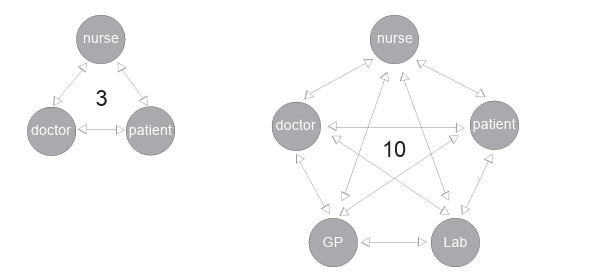
\includegraphics[width=\linewidth]{../graphics/Number-of-conversations.png}
  \caption{Aantal mogelijke conversaties stijgt samen met het aantal personen dat deelneemt aan communicatie. \autocite[Uit ''Communication Systems in Healthcare'' door][The Clinical Biochemist Reviewss, 27(2), 90. Copyright 2006 van \citeauthor{Coiera2006}]{Coiera2006}}
  \label{fig:aantal conversaties}
\end{figure}

\section{\IfLanguageName{dutch}{Onderzoeksvraag}{Research question}}%
\label{sec:onderzoeksvraag}

Het is de combinatie van de stijging in complexiteit van informatie uitwisselen met de nadelen van het \gls{dect}-systeem en de gevaren van alarmmoeheid die ervoor zorgen dat het huidige systeem wordt in vraag getrokken. Zo bekomen we ook de hoofdvraag die wordt behandeld in deze bachelorproef: \textit{''Hoe kan de informatie-uitwisseling tussen artsen en verplegendpersoneel in ziekenhuizen verbeterd worden door het inzetten van nieuwe technologieën''}.\\

\begin{enumerate}
  \item \textit{Wat zijn de kenmerken van het \gls{dect}-\\systeem?}
  \item \textit{Wat is het huidige systeem (met \hyphenation{rand-apparatuur}randapparatuur) en wat zijn de nadelen hiervan?}
  \item \textit{Hoe kan een zorgsituatie worden gesimuleerd?}
\end{enumerate}

Deze bachelorproef zal focussen op het onderzoeken van welke innovaties een waardevol alternatief kunnen zijn voor het \gls{dect}-systeem. Dit onderzoek is gericht op IT-personeel in gezondheidszorginstituten.\\\\

Om een antwoord te formuleren op de hoofdvraag zullen er tussenstappen worden genomen. Deze tussenstappen zijn opgesteld als deelvragen:

\begin{enumerate}
  \item \textit{Welke pogingen zijn al ondernomen om het \gls{dect}-systeem als standaard?}
  \item \textit{Wat zijn de minimumvereisten voor technologieën, om als alternatief te kunnen \\worden beschouwd?}
  \item \textit{Welke andere communicatiemogelijkheden zijn er die voldoen aan de minimumvereisten?}
  \item \textit{Welke mogelijke data-integratiemogelijkheden hebben de alternatieven?}
  \item \textit{Welke eigenschappen van het alternatief hebben een vermindering in alarmmoeheid als gevolg?}
  \item \textit{Vanaf wanneer is het haalbaar om te implementeren op economisch vlak?}
\end{enumerate}

\section{\IfLanguageName{dutch}{Onderzoeksdoelstelling}{Research objective}}%
\label{sec:onderzoeksdoelstelling}

%TODO:

Het beoogde resultaat van deze bachelorproef zijn 2 \gls{poc}'s. Deze bestaan uit een simulatie en een omzetting va nde simulatie naar praktische realisatie. De criteria voor succes zijn de minimum requirements, zie hoofdstuk~\ref{ch:minReq}.
Wat is het beoogde resultaat van je bachelorproef? Wat zijn de criteria voor succes? Beschrijf die zo concreet mogelijk. Gaat het bv.\ om een proof-of-concept, een prototype, een verslag met aanbevelingen, een vergelijkende studie, enz.

\section{\IfLanguageName{dutch}{Opzet van deze bachelorproef}{Structure of this bachelor thesis}}%
\label{sec:opzet-bachelorproef}


De proof of concept die wordt opgesteld tijdens de bachelorproef is in samenwerking met Citymesh en met 360° Zorglab. Citymesh is een bedrijf dat zich specialiseert in connectiviteit, met focus op permanente en tijdelijke netwerkinfrastructuur. Dit door gebruik te maken van WiFi, 0G-, 4G- en 5G-technologieën. \autocite{Citymesh2024} Het 360° Zorglab is een project van HOGENT. De kern van het Zorglab is het creëren van een wisselwerking tussen disciplines enerzijds en tussen onderzoek, dienstverlening en onderwijs anderzijds. Toekomstige gezondheids- en welzijnsmedewerkers kunnen hier in een veilige omgeving niet-technische skills aanleren in een interprofessionele context. \autocite{HOGENT2024} Het doel van deze samenwerking is een snelle wisselwerking te kunnen creëren om zo meerdere malen de testfases te kunnen doorlopen. 

% Het is gebruikelijk aan het einde van de inleiding een overzicht te
% geven van de opbouw van de rest van de tekst. Deze sectie bevat al een aanzet
% die je kan aanvullen/aanpassen in functie van je eigen tekst.

De rest van deze bachelorproef is als volgt opgebouwd:

In Hoofdstuk~\ref{ch:stand-van-zaken} wordt een overzicht gegeven van de stand van zaken binnen het onderzoeksdomein, op basis van een literatuurstudie.\\

In Hoofdstuk~\ref{ch:methodologie} wordt de methodologie toegelicht en worden de gebruikte onderzoekstechnieken besproken om een antwoord te kunnen formuleren op de onderzoeksvragen.\\

In Hoofdstuk~\ref{ch:minReq} wordt de minimumvereisten verder uitgediept. Dezer zijn opgesteld aan de hand van eisen van ziekenhuizen, co-promotoren en gebreken van het \gls{dect}-systeem. Eenmaal alle vereisten zijn uitgeklaard, worden de vooropgestelde technologieën geevalueerd ten opzichte van deze vereisten.\\

In Hoofdstuk~\ref{ch:poc1} wordt de eerste \gls{poc} uitgelegd en aangetoond hoe deze tot stand is gekomen met de code. Deze zal ook in dit hoofdstuk worden geevalueerd en een tussentijds resultaat zal worden opgesteld.\\

In Hoofdstuk~\ref{ch:poc2} wordt de tweede \gls{poc} opgesteld. Deze is een evolutie van de eerste \gls{poc}, van simulatie naar realisatie on site in het 360° zorglab.\\

In Hoofdstuk~\ref{ch:financieel} wordt er een algemeen overzicht gemaakt van de tweede \gls{poc}, met een schatting voor het opschalen voor grotere sites.\\

In Hoofdstuk~\ref{ch:controle} wordt er gecontroleerd of de tweede \gls{poc} voldoet aan de vooropgestelde minimumvereisten uit hoofdstuk~\ref{ch:minReq}. \\

In Hoofdstuk~\ref{ch:conclusie}, tenslotte, wordt de conclusie gegeven en een antwoord geformuleerd op de onderzoeksvragen. Daarbij wordt ook een aanzet gegeven voor toekomstig onderzoek binnen dit domein.
\chapter{\IfLanguageName{dutch}{Stand van zaken}{State of the art}}%
\label{ch:stand-van-zaken}

% Tip: Begin elk hoofdstuk met een paragraaf inleiding die beschrijft hoe
% dit hoofdstuk past binnen het geheel van de bachelorproef. Geef in het
% bijzonder aan wat de link is met het vorige en volgende hoofdstuk.

% Pas na deze inleidende paragraaf komt de eerste sectiehoofding.

De huidige stand van zaken kan worden opgedeeld in 5 delen. Het eerste deel is een situatieschets van de huidige complete set-up van het \gls{dect}-systeem, met al zijn gebreken en voordelen. Deze voor- en nadelen worden dan verwerkt in het 2de deel. Hierin wordt er een oplijsting gemaakt waaraan de nieuwe / vervangende technologieën aan moeten voldoen. Het overzicht is opgesteld via de MoSCoW techniek. Vervolgens is er een oplijsting van mogelijke alternatieven voor het \gls{dect}-systeem gevolgd door een uitdieping van de alternatieven hun eigenschappen en mogelijke gebruik. Om na de uiteenzetting afgetoetst te worden aan de requirements. Als voorlaatste deel wordt er gekeken naar de data en de implicatie hiervan. Dit hoofdstuk wordt afgesloten met een uiteenzetting van het huidige  securitylandschap.

\section{\IfLanguageName{dutch}{\gls{dect}-systeem}{\gls{dect}-system}}%
\label{sec:dect-systeem}
Het \gls{dect}-systeem staat voor Digital Enhanced Cordless Telecommunications; dit is een standaard in de EU sinds 1993. De meest gebruikte situatie is waar er meerdere gebruikers zijn voor een draadloze communicatie in werkomgevingen. De voornaamste reden voor gebruik van het draadloos \gls{dect}-systeem is dat het een grote dichtheid van veel gebruikers aankan \autocite{Welinder1997}. In vergelijking met andere mobiele communicatiesystemen werkt het niet buiten de werkomgeving \autocite{Welinder1997}. Na onderzoek van \textcite{Welinder1997} bleek dat de interferentie van het \gls{dect}-systeem op medisch gereedschap 11 procent was. De interferentie valt echter volledig weg bij een afstand van 0,5m tussen het gereedschap en het \gls{dect}-toestel. \\
Verder heeft het \gls{dect}-systeem volgens \textcite{Welinder1997}een hoge betrouwbaarheid, een groot bereik binnen gebouwen, lage energieconsumptie en een eigen frequentieband.
Deze frequenties liggen tussen 1880 MHz en 1900 MHz, opgesplitst in 10 kanalen. De kanalen op zich bestaan elk uit 12 duplex tijdsloten, dit resulteert in 120 bruikbare radiokanalen \autocite{ETSI1999}. Hoewel het \gls{dect}-systeem een standaard is sinds 1993, zijn er toch verschillende innovaties toegepast op dit systeem, maar deze worden als een apart systeem of technologie gezien. \\
Het is belangrijk ook om te vermelden dat in deze bachelorproef enkel Intra-ziekenhuis communicatie wordt onderzocht. Dit betekent dat enkel binnen eenzelfde site wordt gekeken om een oplossing of alternatief te bieden voor het \gls{dect}-systeem.

\section{\IfLanguageName{dutch}{Vereisten}{Requirements}}%
\label{sec:req}%


%---------

% Volgens \textcite{Coiera2006} zijn volgende aspecten van een communicatiesystemen voor ziekenhuizen van uiterst belang:

% \begin{enumerate}
%     \item Betrouwbaarheid en Beschikbaarheid
%     \item Beveiliging en Privacy
%     \item \acrfull{qos}
%     \item Interoperabiliteit
%     \item Mobilitetit en Dekking
%     \item Schaalbaarheid
%     \item Gebruiksvriendelijkheid
%     \item Integratie met (huidige) klinische workflows 
% \end{enumerate}

% Verder wordt er met het oog op de toekomst ook extra requirements toegevoegd. Deze zijn de volgende:

% \begin{enumerate}
%     \item Beschikbaarheid van Data
%     \item Prioritisering
% \end{enumerate}

% \textbf{DIT HOOFDSTUK ZAL WORDEN AANGEVULD TEGEN DE 2DE DEADLINE (SEMESTER 2)}

% \section{\IfLanguageName{dutch}{Betrouwbaarheid en Beschikbaarheid}{Reliability and Availability}}
% \label{sec:betrouwbaarheid-en-beschikbaarheid}
%


% \section{\IfLanguageName{dutch}{Beveiliging en Privacy}{Security and Privacy}}
% \label{sec:beveiliging-en-privacy}
%



% \section{\IfLanguageName{dutch}{Quality of Service}{Quality of Service}}
% \label{sec:quality-of-service}
%



% \section{\IfLanguageName{dutch}{Interoperabiliteit}{Interoperability}}
% \label{sec:interoperabiliteit}
% 



% \section{\IfLanguageName{dutch}{Mobilitetit en Dekking}{Mobility and Coverage}}
% \label{sec:mobilitetit-en-dekking}
% 



% \section{\IfLanguageName{dutch}{Schaalbaarheid}{Scalability}}
% \label{sec:schaalbaarheid}
% %



% \section{\IfLanguageName{dutch}{Gebruiksvriendelijkheid}{User-friendly Interface}}
% \label{sec:gebruiksvriendelijkheid}
%



% \section{\IfLanguageName{dutch}{Integratie met (huidige) klinische workflows}{Integration with Clinical Workflows}}
% \label{sec:integratie-met-klinische-workflows}
%
%---------
Voor de vereisten of requirements wordt er gebruik gemaakt van de MoSCoW techniek. Dit is een prioritatie techniek uit het Agile framework. Volgens \textcite{2025agile} staan de letters voor:

\begin{itemize}
  \item \textbf{M}ust have - Noodzakelijk
  \item \textbf{S}hould have - Duidelijke meerwaarde
  \item \textbf{C}ould have - Niet-noodzakelijke meerwaarde
  \item \textbf{W}on't have this time - Niet in deze versie
\end{itemize}

Als er dan dieper wordt gekeken naar deze opdeling kan men bij elke categorie een verduidelijking plaatsen. Zo stelt \textcite{2025agile}:\\

\textbf{\textit{Must have}} bestaat uit de minimale oplijsting van vereisten die nodig zijn om het project te kunnen opleveren. Dit houdt in dat er gekeken wordt naar wetten, veiligheid, wat er als 'bare-minimum' moet zijn.\\

\textbf{\textit{Should have}} wordt beschreven als belangrijk maar niet noodzakelijk. Het project kan bestaan zonder, maar mogelijke workarounds zijn nodig ald dan niet tijdelijk.\\

\textbf{\textit{Could have}} zijn zaken die een meerwaarde kunnen bieden, maar een minimale impact hebben indien niet geïmplementeerd. Het verschil tussen should en could have ligt in de gradatie van problemen/pijn veroorzaakt indien er niet aan de vereiste wordt voldaan.\\

\textbf{\textit{Won't have}}, vereisten die op het eerste zich interessant zijn maar de laagste prioriteit krijgen. Dit is geen onderdeel van het huidige product/project, maar kan in de toekomst met een revisie worden geïmplementeerd.\\

\subsection{Must have}
\label{sec:Must-have}

\begin{itemize}
  \item Wetgeving conform
  \subitem \gls{ehds}
  \subitem \gls{nis2}
  \subitem \gls{gdpr}
  \item Gesloten systeem
  \item Stabiel
  \item Segregatie 
  \item Communicatie eisen
\end{itemize}

Volgens \textcite{Coiera2006} zijn de volgende zaken vereist om te spreken van een communicatiesysteem:
\begin{itemize}
  \item Communicatiekanaal
  \item Boodschap
  \item Communicatiebeleid
  \item Communicatietoestel
  \item Interacties
  \item Beveiligingsbeleid
\end{itemize}

\subsection{Should have}
\label{sec:Should-have}

\begin{itemize}
  \item Opties voor meer dan enkel audiocommunicatie
\end{itemize}

\subsection{Could have}
\label{sec:Could-have}

\begin{itemize}
  \item Interne data gebruik mogelijk
  \item Monitoring software voor audits van het systeem
  \item AI controle systeem
\end{itemize}

\subsection{Won't have}
\label{sec:Wont-have}

\begin{itemize}
  \item Integratie medische apparatuur
  \item Monitoring software voor audits van het systeem
\end{itemize}

\section{\IfLanguageName{dutch}{Andere communicatietechnologieën}{Other communication Technologies}}%
\label{sec:andere}%

Op basis van studies van \textcite{Montalvo2024}, \textcite{Kranz2010} en \textcite{Soenmez2018} kan er een lijst worden opgesteld van alternatieven voor het \gls{dect}-systeem:

\begin{itemize}
  \item \gls{lte} Advanced
  \item 5G
  \item \gls{ule}
  \item \gls{voip}
\end{itemize}

Elke technologie wordt besproken op eenzelfde manier. Eerst wordt de techniek verklaard, vervolgens wordt de functionaliteit uitgeklaard. Eens deze duidelijk zijn wordt de technologie afgetoetst op de vereisten.

\subsection{\IfLanguageName{dutch}{\gls{lte} Advanced}{\gls{lte} Advanced}}%
\label{sec:ltea}%

\gls{lte} of Long Term Evolution is de overkoepelende technologie waaronder 5G valt. Volgens \textcite{Bakare2022} is ook een verbetering van \gls{lte} Advanced, een stap naar de toekomst van \gls{lte}. De voornaamste eigenschappen van \gls{lte} Advanced zijn, opgelijst door \textcite{Bakare2022}:

\begin{itemize}
  \item Drie keer beter in spectrumefficiëntie in vergelijking met \gls{lte}
  \subitem 30 bps/Hz downlink
  \subitem 15 bps/Hz uplink
  \item Datapiek 
  \subitem 1 Gbps downlink
  \subitem 500 Mbps uplink
  \item Ondersteuning voor schaalbare bandbreedte en spectrumaggregatie
  \item Lage latentie
  \item Zeer goede compatibiliteit met \gls{lte}
\end{itemize}

\subsection{\IfLanguageName{dutch}{5G}{5G}}%
\label{sec:5g}%
5G is een stap in de evolutie van het mobiele netwerk, opvolger van 4G. In deze bachelorproef gaat het om het private 5G-netwerk. Volgens \textcite{wen2021private} zijn er eigenschappen van private 5G die nauw aansluiten met die van \gls{dect}-systemen. De eerste eigenschap wijst op de hoge apparatuurdichtheid, maar bij 5G gaat deze ook nog eens gepaard met hoge throughput. Dit zorgt voor integratie van externe devices, zoals sensoren, camera's, etc. . Vervolgens heeft 5G ook voordelen ten opzichte van \gls{dect}-systemen volgens \textcite{wen2021private}. Zo is er een hoge betrouwbaarheid met een lage latency. Deze lage latency geeft nieuwe mogelijkheden, zoals bv. een chirurgische ingreep vanop afstand.\\ De tweede eigenschap van het privaat netwerk is de flexibiliteit en voorspelbaarheid van \gls{qos}. Daarnaast zijn er verschillende architecturen die men kan implementeren om een privaat 5G-netwerk op te zetten. De eerste methode is een standalone deployment. Hierbij wordt een privaat netwerk opgezet, waarbij alle netwerk functies van het netwerk zijn gelimiteerd binnen een logische perimeter bestaande uit vooraf gedefinieerde regio's. De andere methode is een publiek netwerk geïntegreerd deployment. Deze architectuur kan worden opgesplitst in verschillende types, afhankelijk van de gradatie van integratie. Deze 4 types zijn de volgende:

\begin{itemize}
  \item \gls{o-ran}
  \item Gedeelde \gls{ran}
  \item Gedeelde \gls{ran} en controle vlak
  \item Gehost bij het Publieke Netwerk
\end{itemize}

\textcite{wen2021private} vermeldt ook dat er naast architectuur een keuze moet worden gemaakt voor het spectrum. Hier zijn ook opnieuw 3 keuzes: een specifiek privaat spectrum, een erkend spectrum en een niet-erkend spectrum. 
5G heeft een aantal noodzakelijke technologieën nodig in het netwerk. Een van deze technologieën is network slicing. Hierbij wordt er 'een netwerk in een netwerk' gemaakt door het fysieke netwerk op te splitsen in meerdere logische netwerken. Om aan network slicing te kunnen doen, is er een nood aan netwerk-virtualisatie. Het slicing zelf kan worden opgedeeld in 3 lagen: Infrastructuurlaag, Network-slice laag en Onderhoudslaag. De levensloop van het slicen van een netwerk verloopt volgens de volgende 4 fases \autocite{wen2021private}:

\begin{enumerate}
  \item Voorbereiding
  \item In dienst stellen
  \item Gebruik
  \item Ontmanteling
\end{enumerate}


\subsubsection{\IfLanguageName{dutch}{Publiek versus privaat}{Public versus private}}
\label{public-v-private}

Binnen België is het 5G spectrum door overheid vastgelegd. Volgens \textcite{Eede2023} zijn er 3 delen op het 5G spectrum:\\\\
Het eerste deel is een non-licensed deel, dit betekent dat dit vrij is voor iedereen. Dit deel ligt tussen de 2,40 en de 2,48 GHz. Op de deel van het 5G spectrum werkt onder andere WLAN, Bluetooth en ZigBee.\\
Het tweede deel wat wordt beheerd door de telecom providers.

\begin{table}[H]
\centering
\begin{tabular}{|l|l|l|}
\hline
\textbf{3600MHz-band}      & \textbf{Bandbreedte} & \textbf{Frequentiebereik}    \\ \hline
Citymesh Mobile nv         & 50 MHz               & 3430--3480 MHz               \\ \hline
PROXIMUS                   & 20 MHz               & 3580--3600 MHz               \\ \hline
Orange Belgium nv          & 100 MHz              & 3600--3700 MHz               \\ \hline
Proximus nv                & 100 MHz              & 3700--3800 MHz               \\ \hline
Telenet Group nv           & 100 MHz              & 3480--3580 MHz               \\ \hline
\end{tabular}
\caption{5G verdeling onder telecom providers. \autocite[Door]{Eede2023} [ Copyright 2023 van \textcite{Eede2023}}
\end{table}


Tenslotte is er het laatste deel gereserveerd voor het 5G private netwerk.  Dit ligt tussen de 3,80 en de 4,20 GHz, wat betekend dat er 40 MHz beschikbaar is voor het private netwerk.


\subsubsection{\IfLanguageName{dutch}{Frameworks}{Frameworks}}
\label{framework}

Er zijn verschillende frameworks beschikbaar, maar met de focus op een toegankelijke methode zal er voornamelijk gefocust worden op open source frameworks. Zo lijst \textcite{Eswaran2022} de verschillende variaties op een open source 5G-framework voor private 5G-netwerken op:

\begin{itemize}
  \item Magma
  \item 5G OpenRAN
  \item ONF's Aether platform
  \item ETSI OSM
  \item \gls{srsRAN}
  \item OpenAirInterface \gls{ue}
\end{itemize}

Na verder onderzoek wordt ook \gls{open5gs} toegevoegd aan deze lijst.\\

Volgens \textcite{Open5GS2024} is Open5G 'een geavanceerd open source project ontworpen voor het bouwen en onderhouden van je eigen NR/\gls{lte} mobiele netwerk. Open5G biedt een robuuste oplossing voor het configureren van zowel \gls{5gnr} als \gls{lte} (Evolved) netwerken.' \\ Verder zijn er andere concepten zoals \gls{o-ran}, waar onder andere het OpenCare5G-netwerk op gebaseerd is. In dit framework wordt Open RAN in een privaat netwerk gebruikt voor digitale gezondheidsapplicaties. Zo hebben \textcite{de2023opencare5g} onderzocht hoe dit framework kan gebruikt worden om gezondheidsonderzoeken te doen met draagbare ultrasone gereedschappen op verschillende locaties. Om deze onderzoeken te kunnen delen met artsen, werd er een lokaal privaat netwerk opgezet. Zo gebruikten ze een 5G xHaul ORAN \gls{oam} privaat netwerk. Er wordt gekozen om een top-down systeem te gebruiken. Dit is een georganiseerde manier om een netwerk project te ontwikkelen. Dit komt doordat men kan steunen op het OSI-model en het 5G-\gls{ran} protocol layer model. Dit zal ook gebruikt worden bij de methodologie. Zo zal er een analyse zijn van elke laag van de 5G-architectuur. Deze architectuur begint met de service laag. Op deze laag komen de verzoeken van de applicatie vandaan. De architectuur eindigt met de infrastructuurlaag. \autocite{de2023opencare5g}

\subsubsection{\IfLanguageName{dutch}{Simulatie}{Simulation}}
\label{sec:open5gs}

Alvorens er wordt gekeken naar \gls{open5gs}, moet er een opsplitsing worden gemaakt in de 5G realisatie.
Zo bestaan er volgens \textcite{Lee2025a} 2 type 5G Cores:

\begin{itemize}
  \item 5G \gls{nsa} vereist een 4G topologie als backbone
  \item 5G \gls{sa}, is een systeem dat zonder andere netwerken kan werken.
\end{itemize}

Hieronder is een figuur die het hele 4G-/ 5G netwerk omvat. De reden dat 4G toch wordt vermeldt in dit schema, is omdat de 5G \gls{nsa} topologie een 4G backbone nodig heeft. \autocite{Lee2025a}

\begin{figure}[H]
  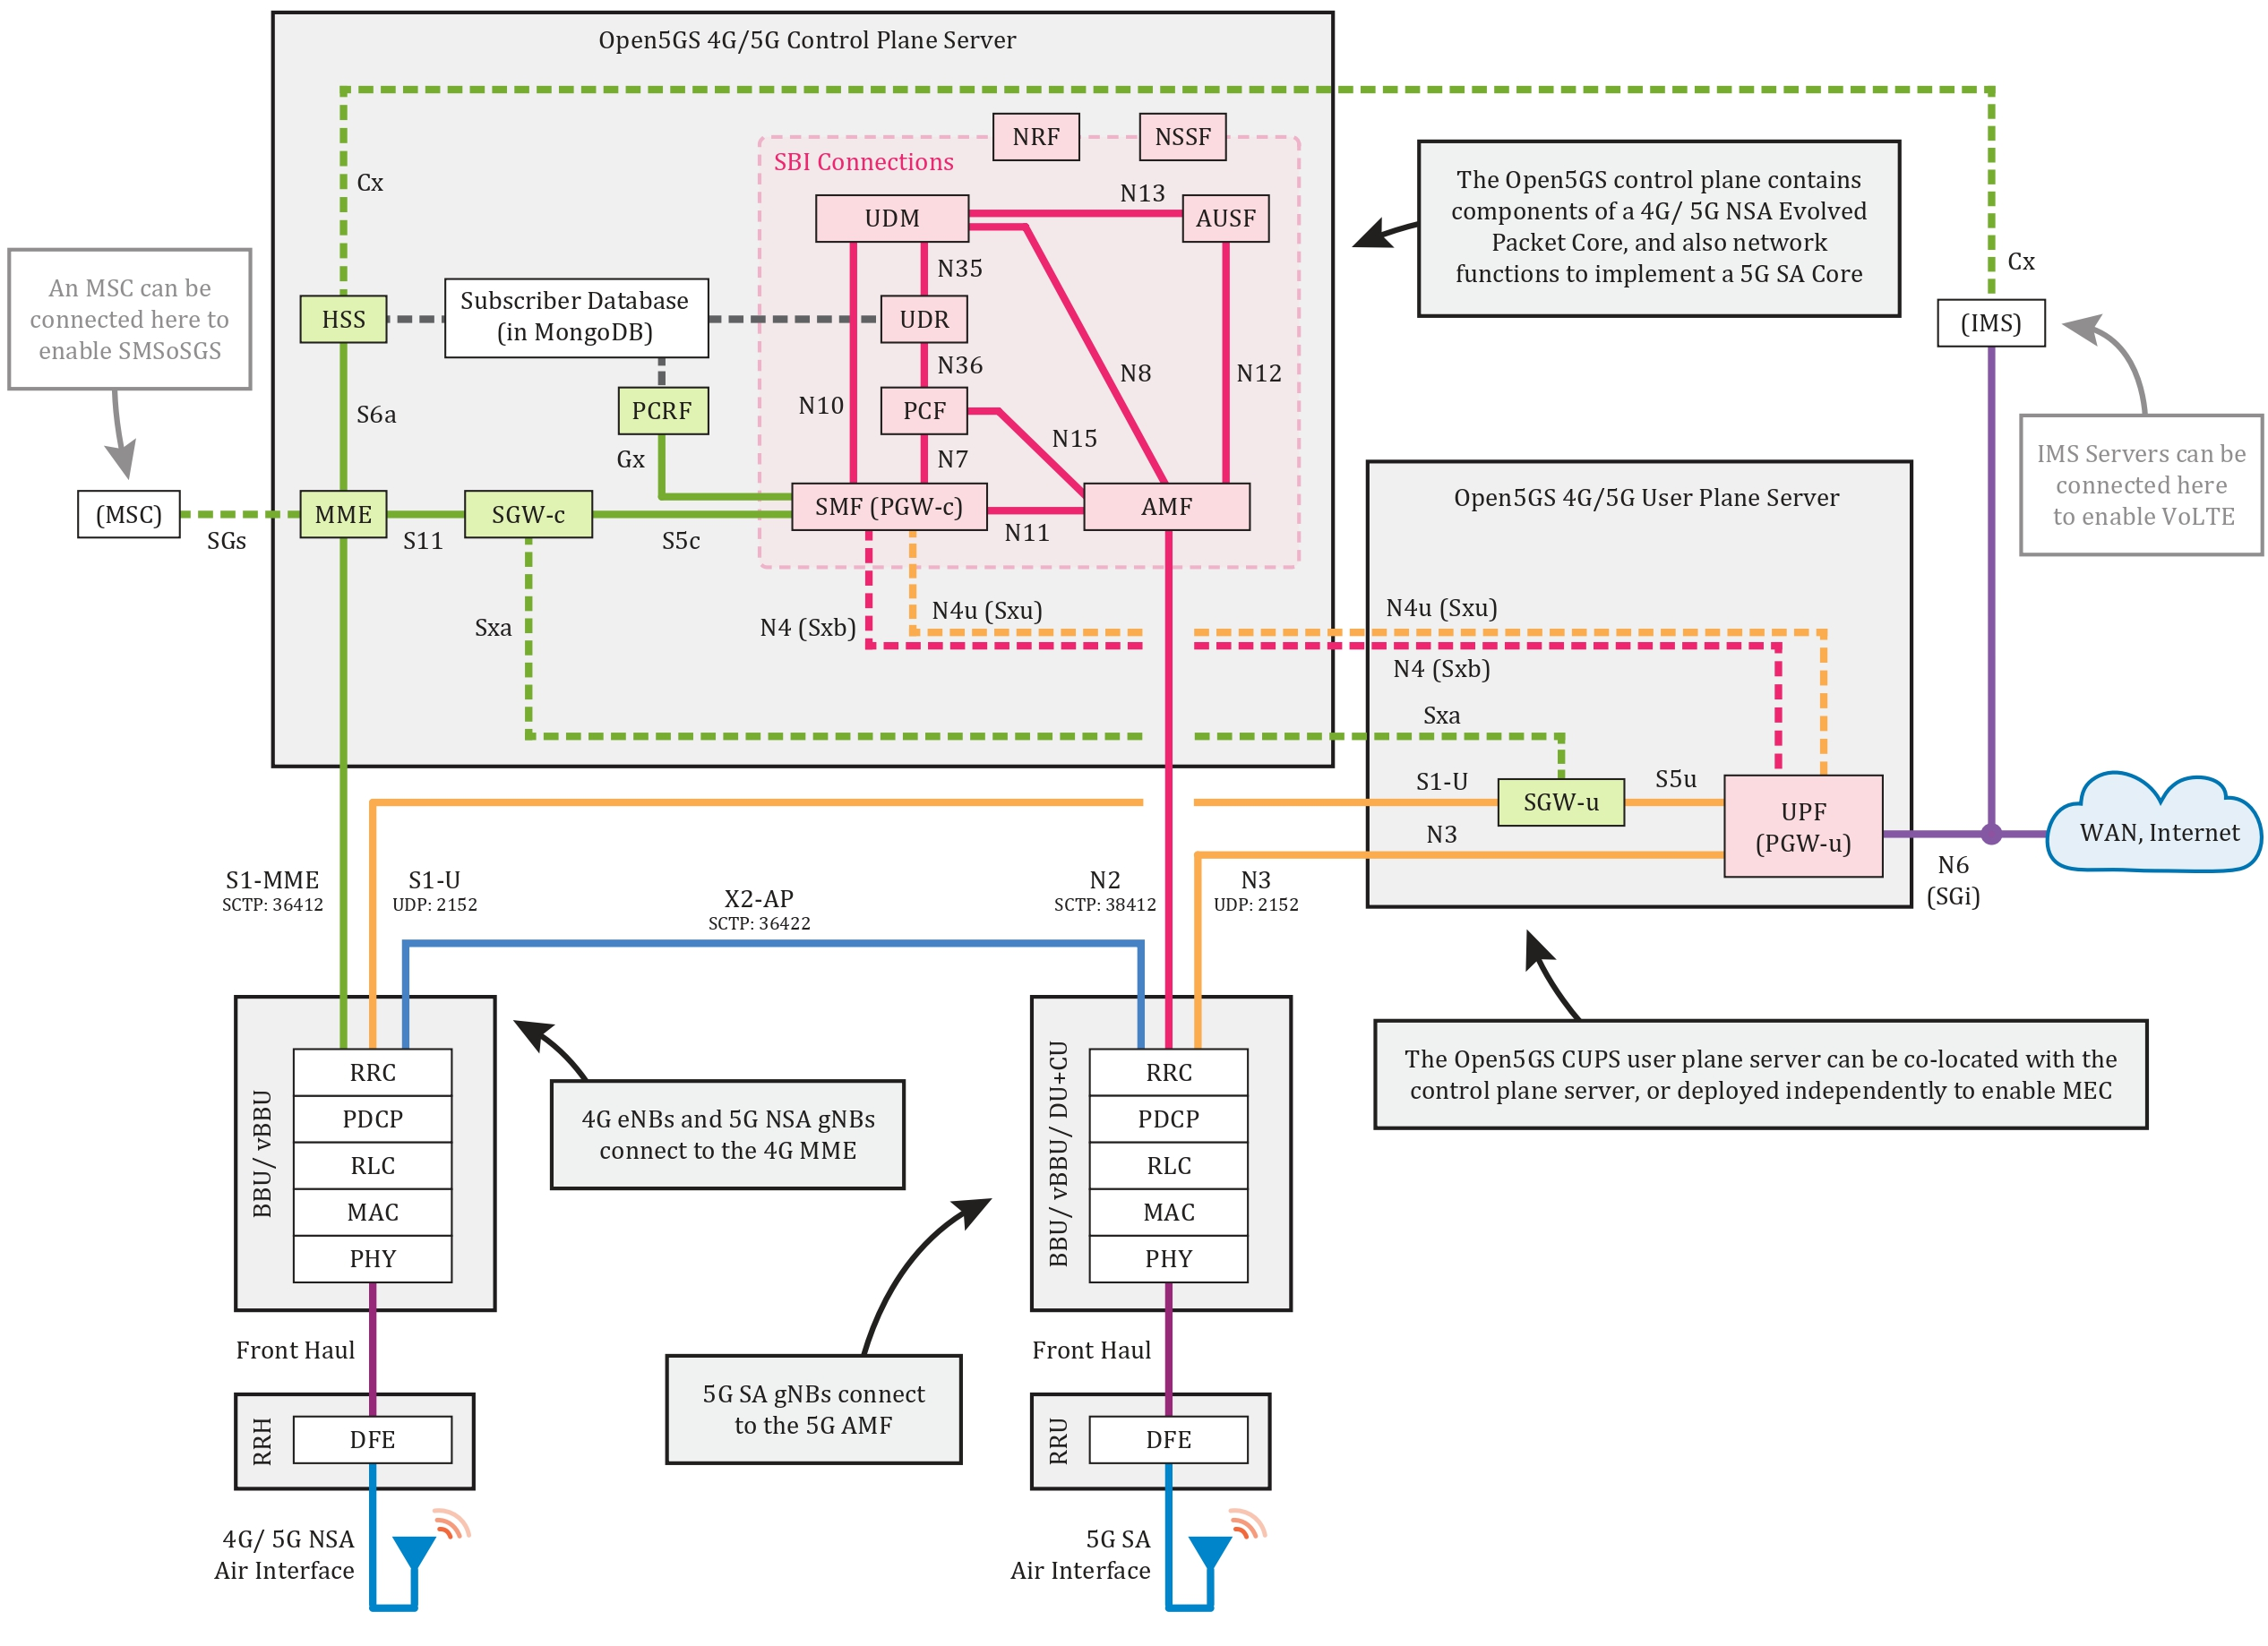
\includegraphics[width=\linewidth]{../graphics/Open5GS-Schema.jpg}
  \caption{Gesimuleerd 5G-netwerk met Open5GS. \autocite[Door][]{Lee2021} Copyright 2021 van \textcite{Lee2021}}
  \label{fig:open5gs-schema}
\end{figure}

\textbf{5G \gls{nsa} Core}\\\\
Volgens \textcite{Lee2025a} heeft de 5G \gls{nsa} Core volgende functies:

\begin{itemize}
  \item \gls{mme}
  \item \gls{hss}
  \item \gls{pcrf}
  \item \gls{sgwc}
  \item \gls{sgwu}
  \item \gls{pgwc-smf}
  \item \gls{pgwc-upf}
\end{itemize}

\textbf{5G \gls{sa} Core}\\\\
Volgens \textcite{Lee2025a} heeft de 5G \gls{nsa} Core volgende functies:

\begin{itemize}
  \item \gls{nrf}
  \item \gls{scp}
  \item \gls{sepp}
  \item \gls{amf}
  \item \gls{smf}
  \item \gls{upf}
  \item \gls{ausf}
  \item \gls{udm}
  \item \gls{udr}
  \item \gls{pcf}
  \item \gls{nssf}
  \item \gls{bsf}
\end{itemize}

Verder stelt \textcite{Lee2025a} ook dat 5G \gls{sa} gebruik maakt van een \gls{sba}. Dit betekent dat een duidelijke scheiding is tussen de Control Plan functies, geregistreerd in de \gls{nrf}, en de User Plane. Deze laatste bevat maar \'e\'en functie, namelijk de \gls{upf}.

Aangezien de simulatie via \gls{open5gs} wordt gedeployd en gekeken wordt vanuit een vervanging van het \gls{dect}-systeem, zal er geopteerd worden voor een 5G \gls{sa} Core. Om deze manier moet er niet eerst een 4G netwerk worden opgezet.

Verder zullen de \gls{gnb} en \gls{ue} worden gesimuleerd met \gls{ueransim}. Dit is ook een bijdragende factor voor de keuze voor de \gls{sa} opstelling, aangezien \gls{ueransim} enkel met dit type netwerken kan werken. Het is wel belangrijk om te vermelden dat \gls{ueransim} geen actieve ontwikkeling meer kent.

\subsubsection{\IfLanguageName{dutch}{Slicing}{Slicing}}
\label{sec:Slicing}

%Foukas2017
%Lorincz2024
%

Volgens \textcite{Foukas2017} zijn er 3 use cases voor slicing:

\begin{itemize}
  \item Versterkte mobiele bandbreedte (\gls{embb})
  \item Massieve machine communicatie
  \item Kritische communicatie
\end{itemize}

Verder stelt \textcite{Lorincz2024} dat er 5 technologieën die netwerk slicing toelaten:

\begin{enumerate}
  \item \gls{sdn} gebaseerd netwerk slicing
  \item \gls{vnf} gebaseerd netwerk slicing
  \item \gls{ran} gebaseerd netwerk slicing
  \item Netwerk slicing gebaseerd op de aanpassing vna het netwerkverkeer aan de patronen van energieverbruik
  \item \gls{e2e} netwerk slicing met strikte beveiligings vereisten
\end{enumerate}

\begin{figure}[H]
  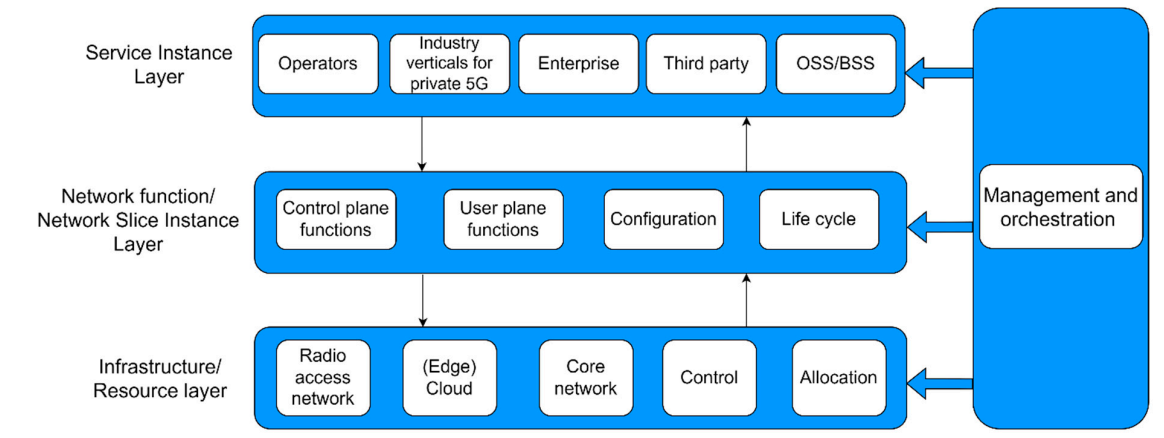
\includegraphics[width=\linewidth]{../graphics/slice.png}
  \caption{Concept van 5G netwerk slicing \autocite[Door][]{Lorincz2024} Copyright 2024 van \textcite{Lorincz2024}}
  \label{fig:slice}
\end{figure}

\textcite{Lorincz2024} gaat verder met verklaren dat elke \gls{ns} in een 5G netwerk ook een uniek kan worden geidentificeerd worden door middel van \gls{s-nssai}. Deze identifier wordt gebruikt in communicatie tussen \gls{ue} en het 5G netwerk. De \gls{s-nssai} bestaat uit een 8-bit \gls{sst-id} en een 24-bit \gls{sd}, deze laatste is een optionele parameter. De huidige gestandaardiseerde \gls{sst-id}'s zijn de volgende:

\begin{itemize}
  \item \gls{embb}
  \item \gls{urllc}
  \item \gls{miot}
  \item \gls{v2x}
  \item \gls{hmtc}
  \item \gls{hdllc}
\end{itemize}

Gezien de context van een ziekenhuis omgeving en het doel een vervanging is van het \gls{dect}-systeem zal enkel worden gekeken naar de \gls{sst-id} types die betrekking hebben tot direct communicatie en noodgevallen. Dit zijn de eerste twee: \gls{embb} en \gls{urllc}.

Implementatie van \gls{embb} slices is toepasbaar op het huidgie mobiele netwerk en kan uitgebreid wordemn naar mogelijke andere doeleinden van dat netwerk voor een volledig intmnet elkaar verbonden maatschappij. \autocite{Lorincz2024}

De \gls{urllc} services zijn gekenmerkt door de nood om directe interactie te hebben. 

Het is wel belangrijk om rekening te houden met het feit dat deze twee \gls{sst-id}'s een hoge energieconsumptie hebben in vergelijking met de andere \gls{sst-id}'s. Dit komt door de grote en frequente intensiteit van het dataverkeer dat kararkteristiek is aan \gls{embb} en \gls{urllc} slices. \autocite{Lorincz2024}

Verder is het ook niet altijd mogelijk om aan slicing te kunnen doen. Daarom worden er ook alternatieven binnen het 5G netwerk voor slicing gebruikt. Er wordt dan gebruik gemaakt van \gls{ddn}. Dit is een vaak gebruikt alternatief voor slicing van ee n5G netwerk aangezien er een apart data netwerk wordt opgezet. Dit is echter qua veiligheid niet hetzlefde als volwaardige slicing waar een identifier (\gls{s-nssai}). Het gebruiken van \gls{ddn} is een opvolger van het \gls{APN}, dit doet exact hetzelfde maar specifiek voor 4G netwerken \autocite{Eede2023}.

\subsubsection{\IfLanguageName{dutch}{Kosten}{Costs}}
\label{sec:Cost}

Volgens \textcite{Abbas2024} is er een grotere kost dan enkel de aankoop van de installatie. Zo zijn er voor elke fase van het 5G installatie-project vaak verdoken kosten:

\begin{itemize}
  \item Planning kost
  \item Licentie kost 
  \item Infrastructuur kost (Hardware)
  \item Implementatie kost
  \item onderhoudskosten
  \item Use case kost (Opzetten van het project)
\end{itemize}

Zo verduidelijkt \textcite{Abbas2024} dat er in de implementatie fase al redelijk wat verdoken kosten zitten, zoals hieronder aangetoond.
\begin{figure}[H]
  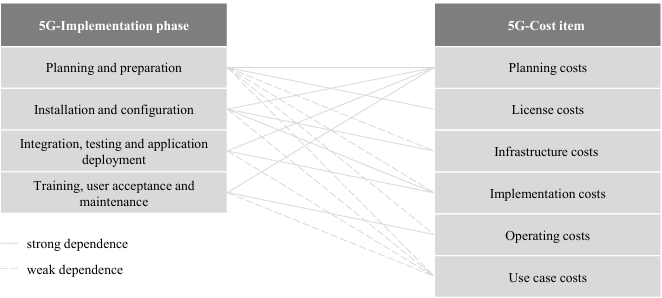
\includegraphics[width=\linewidth]{../graphics/kost-associaties.png}
  \caption{Afhankelijkheden tussen implementatie fase en kosten \autocite[Door][]{Abbas2024} Copyright 2024 van \textcite{Abbas2024}}
  \label{fig:Cost}
\end{figure}

Dit wordt ook aangetoond door \textcite{Hilary2024} dat men zich niet alleen mag focussen op de \gls{capex} van de 5G installatie, maar ook de \gls{opex}. Dit wordt nogmaals aangetoond door middel van de staafdiagrammen van \textcite{Hilary2024}

De simulatie die als \gls{poc} wordt gebruikt valt onder de categorie \gls{snpn}. De andere categorieën zijn Legacy 5G netwerken, dit is wat in deze bachelorproef het 5G \gls{nsa} netwerk wordt genoemd. Verder zijn er 2 categorieën die beiden vertrekken van een RAN die gedeeld wordt. Het grootste verschil tussen de beiden is het gebruik van een eigen control plane of niet.

\begin{figure}[H]
  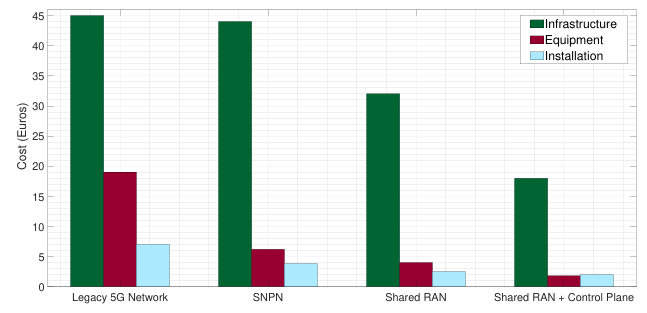
\includegraphics[width=\linewidth]{../graphics/capex.png}
  \caption{\gls{capex} van een 5G netwerk \autocite[Door][]{Hilary2024} Copyright 2024 van \textcite{Hilary2024}}
  \label{fig:capex}
\end{figure}

Dit staafdiagram toont aan dat de \gls{capex} en initiële installatiekost verdeeld wordt in drie subkosten:

\begin{itemize}
  \item Infrastructuur of hardware
  \item Gereedschap
  \item Installatie op zich
\end{itemize}

Hoewel deze kosten varieren tussen het type netwerk dat wordt gedeployd, toch is er een duidelijke trend. Deze is dat de hardware de grootste kost met zich meebrengt.

\begin{figure}[H]
  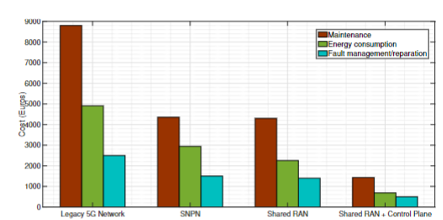
\includegraphics[width=\linewidth]{../graphics/opex.png}
  \caption{\gls{opex} van een 5G netwerk \autocite[Door][]{Hilary2024} Copyright 2024 van \textcite{Hilary2024}}
  \label{fig:opex}
\end{figure}

Vervolgens wordt aangetoond dat de \gls{opex} ook kan worden opgesplitst in drie subkosten:

\begin{itemize}
  \item Onderhoud
  \item Energieconsumptie
  \item Fout management en reparaties
\end{itemize}

Net zoals bij de \gls{capex} is er ook hier weer een trend zichtbaar. Het onderhoud is hier de grootste kost.

\begin{figure}[H]
  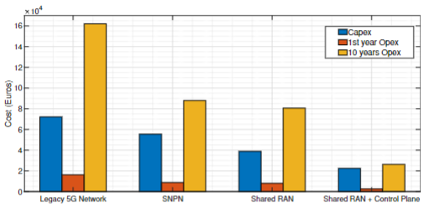
\includegraphics[width=\linewidth]{../graphics/capex-opex.png}
  \caption{Vergelijking van \gls{capex} met \gls{opex} op 1 jaar en op 10 jaar tijd \autocite[Door][]{Hilary2024} Copyright 2024 van \textcite{Hilary2024}}
  \label{fig:capex-vs-opex}
\end{figure}

Als men dan nadien de \gls{capex} met de \gls{opex} (op 1 jaar en op 10 jaar) gaat vergelijken ziet men dat de langetermijn \gls{opex} de uitschieter is. 

\subsection{\IfLanguageName{dutch}{ULE}{ULE}}%
\label{sec:ule}%

\gls{ule} is een uitbreiding op het \gls{dect}-systeem zelf. Volgens \textcite{GariniDil2014} is dit een samenwerking tussen het \gls{dect}-systeem, \gls{cat-iq} (nieuwste HD voice-technologie) en een nieuwste aanpassing van data technologie \gls{ule} (Ultra Low Energy). Aangezien dit een uitbreiding is op het huidige \gls{dect}-systeem is er dus een makkelijke installatie en compatibiliteit.

De grootste voordelen van deze technologie volgens \textcite{GariniDil2014} zijn:

\begin{itemize}
  \item Open wereldwijde standaard
  \item Interferentievrije frequentieband
  \item Verbeterde veilige range
  \subitem Alle communicatie is versleuteld
  \item Lage kost
  \item Video en audio
\end{itemize}

Verder onderzoek door \textcite{Das2012} toont aan dat \gls{ule} ook een goede oplossing is voor de gezondheidszorg. Dit komt door de lage energieconsumptie, de lange levensduur van de batterij en de lage kosten. Dit maakt het een goede kandidaat voor een communicatiesysteem in de gezondheidszorg. Uit de deze studie (\textcite{Das2012}) kan men ook een oplijsting halen waarin verschillende technologieën worden vergeleken met het \gls{dect}-systeem. Dit is te zien in de tabel hieronder.

\begin{figure}[H]
  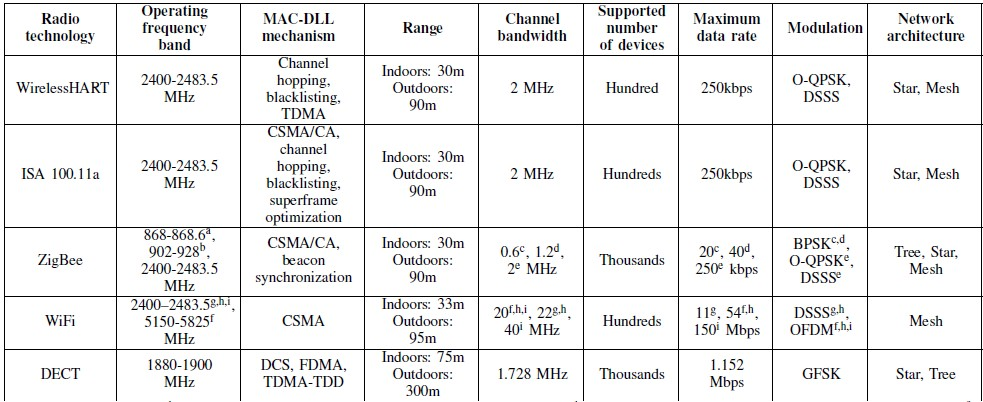
\includegraphics[width=\linewidth]{../graphics/overzicht.jpg}
  \caption{Overzicht gelijkaardige systemen zoals \gls{ule} \autocite[Door][]{Das2012} Copyright 2012 van \textcite{Das2012}}
  \label{fig:overzicht}
\end{figure}


Naast deze tabel, onderzocht \textcite{Das2012} kwaliteit van de kanalen die worden gebruikt door \gls{ule}. Verder wordt er naar de kans dat een kanaal selectie faalt in het \gls{ule}-systeem, de vertraging op communicatie en de gehele performantie van het netwerk onder verschillende belastingen. Hieronder zijn een overzicht van de mogelijke knalen die \gls{ule} kan gebruiken. Deze verschillende kanalen kan worden geïnterpreteerd als het \gls{ule} alternatief voor het 5G slicen.

\begin{figure}[H]
  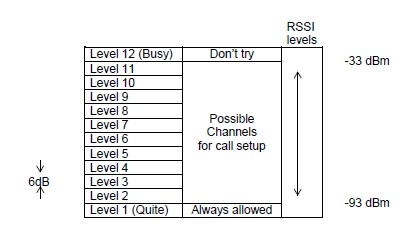
\includegraphics[width=\linewidth]{../graphics/ULE-channels.jpg}
  \caption{Lijst met channel selectie \autocite[Door][]{Das2012} Copyright 2012 van \textcite{Das2012}}
  \label{fig:ule-channels}
\end{figure}

\subsection{\IfLanguageName{dutch}{VoIP}{VoIP}}%
\label{sec:voip}%

\gls{voip} of Voice Communication over the Internet Protocol is een communicatietechnologie dat telefooncommunicatie stuurt over het internet in plaats van het telefoonnetwerk te gebruiken. \Autocite{Soenmez2018} Er zijn 5 scenario's waarin \gls{voip} kan worden gebruikt. Deze worden opgelijst door \textcite{Soenmez2018}:

\begin{itemize}
  \item Computer naar Computer
  \item Computer naar telefoon (\gls{pstn}) (of omgekeerd)
  \item Telefoon (\gls{pstn}) naar Telefoon (\gls{pstn})
  \item Mobiele \gls{voip}
  \item Draadloze \gls{voip}
\end{itemize}

Echter, \textcite{Soenmez2018} bevestigt wel dat er een groot aanvalsoppervlak bestaat. Zo heeft de \gls{voipsa} een lijst gepubliceerd met 6 beveiligingspunten waar countermeasures moeten geïnstalleerd worden om een veilige omgeving te garanderen.

\section{\IfLanguageName{dutch}{Data}{Data}}%
\label{sec:data}%

Volgens \textcite{Niekerk2020} is de gezondheidszorg rijk aan data en is deze data ook nog eens waardevol. Toch wordt er maar 50\% gebruikt.
De data kan een ondersteunende factor zijn om de alarmmoeheid weg te werken. Zo onderzocht \textcite{Hever2019} de mogelijkheid om met data en machine learning de valse alarmen te verminderen. In dat onderzoek werd dit getest op de Intensieve Zorg afdeling. In de conclusie van \textcite{Hever2019} stelt deze dat door het gebruik van deze data er een \gls{ai}-model opgeleid kon worden om de afdeling stiller en betrouwbaarder te maken. Dit verminderde het effect van alarmmoeheid. Verder meldt \textcite{Hever2019} dat door deze data en het model  ontbrekende factoren kunnen interpoleren.

\section{\IfLanguageName{dutch}{Beveiliging}{Security}}%
\label{sec:security}%

In samenspraak met de copromotor is er geopteerd om cybersecurity niet actief te onderzoeken in deze bachelorproef. Echter, het is wel noodzakelijk om te weten dat er verschillende verplichtingen zijn in België en de Europese Unie. Als men een introductie van een 5G-netwerk uitvoert in een gezondheidszorgomgeving en/of ziekenhuizen is er sprake van een vergroting van de 'attack surface'. De beveiliging van dit type omgeving, ook wel de beveiliging van gezondheidszorg 5.0 genoemd, doet een beroep op de \gls{cia}-principes. Echter, \textcite{Wazid2022} voegt nog enkele extra eisen toe:

\begin{itemize}
  \item Beschikbaarheid
  \item Integriteit
  \item Vertrouwelijkheid
  \item Toegangscontrole
  \item Beschikbaarheid
  \item Voorwaartse geheimhouding
  \item Achterwaartse geheimhouding
  \item Onweerlegbaarheid
\end{itemize}

Als al deze principes worden toegepast, kan men stellen dat er voldaan is aan de minimum noodzakelijke beveiliging van het gezondheidszorgsysteem. Zo stelt \textcite{Wazid2022} vier reeds bestaande schema's voorop voor de beveiliging van dit systeem, elk met hun taak, features en beperkingen:

\begin{itemize}
  \item \gls{b2h} \autocite{Ghosh2022}
  \item Blockchain en quantum-blindhandtekening \autocite{Bhavin2021}
  \item Systeembreed sleutelschema \autocite{Chang2022}
  \item \gls{bits} \autocite{Gupta2020}
\end{itemize}
\subsection{\IfLanguageName{dutch}{Wetgevingen}{Laws}}%
\label{sec:wet}%

Sinds 27 april 2016 is de verordening 2016/679 van toepassing. Deze start de \gls{gdpr} (General Data Protection Regulation) in de Europese Unie. De verordening 2016/679 vermeldt dat "regels worden vastgelegd betreffende de bescherming van natuurlijke personen in verband met de verwerking van persoonsgegevens en het vrije verkeer van persoonsgegevens. Het beschermt de grondrechten en de fundamentele vrijheden van natuurlijke personen, met name hun recht op bescherming van persoonsgegeven."\\ (Verordening (EU) 2016/679 van het Europees Parlement en de Raad van 27 april 2016) %\autocite{gdpr2016} 
\\\\
Vervolgens is er ook het \gls{nis2}, een Belgische wet die bedrijven verplichtingen oplegt op het vlak van cybersecurity. "De wet van 26 april 2024 tot vaststelling van een kader voor de cyberbeveiliging van netwerk- en informatiesystemen van algemeen belang voor de openbare veiligheid (de "\gls{nis2}-wet") zet de EU-richtlijn 2022/2555 van het Europees Parlement en de Raad van 14 december 2022 (de "\gls{nis2}-richtlijn") om." \\
(Wet tot vaststelling van een kader voor de cyberbeveiliging van netwerk- en informatiesystemen van algemeen belang voor de openbare veiligheid van 26 april 2024) %\autocite{Belgium2024}
\\\\
Tenslotte is er een nieuwer initiatief genaamd \gls{ehds} (European Healthcare Data Space). Dit initiatief heeft het volgende doel: "De algemene doelstelling is te waarborgen dat natuurlijke personen in de EU in de praktijk meer zeggenschap over hun elektronische gezondheidsgegevens hebben."\\ (Voorstel (EU) COM/2022/197 van het Europees Parlement en de Raad van 3 mei 2022) %\autocite{\gls{ehds}2022}

%%=============================================================================
%% Methodologie
%%=============================================================================

\chapter{\IfLanguageName{dutch}{Methodologie}{Methodology}}%
\label{ch:methodologie}

%% TODO: In dit hoofstuk geef je een korte toelichting over hoe je te werk bent
%% gegaan. Verdeel je onderzoek in grote fasen, en licht in elke fase toe wat
%% de doelstelling was, welke deliverables daar uit gekomen zijn, en welke
%% onderzoeksmethoden je daarbij toegepast hebt. Verantwoord waarom je
%% op deze manier te werk gegaan bent.
%% 
%% Voorbeelden van zulke fasen zijn: literatuurstudie, opstellen van een
%% requirements-analyse, opstellen long-list (bij vergelijkende studie),
%% selectie van geschikte tools (bij vergelijkende studie, "short-list"),
%% opzetten testopstelling/PoC, uitvoeren testen en verzamelen
%% van resultaten, analyse van resultaten, ...
%%
%% !!!!! LET OP !!!!!
%%
%% Het is uitdrukkelijk NIET de bedoeling dat je het grootste deel van de corpus
%% van je bachelorproef in dit hoofstuk verwerkt! Dit hoofdstuk is eerder een
%% kort overzicht van je plan van aanpak.
%%
%% Maak voor elke fase (behalve het literatuuronderzoek) een NIEUW HOOFDSTUK aan
%% en geef het een gepaste titel.
Tijdens het verloop van de bachelorproef zullen er antwoorden worden vergaard op verschillende deelvragen die helpen de onderzoeksvraag te beantwoorden. Zo zal elke deelvraag deel uitmaken van een onderdeel van de methodologie.
\\\\
De bachelorproef verloopt in de volgende fasen:

\begin{figure}[h]
  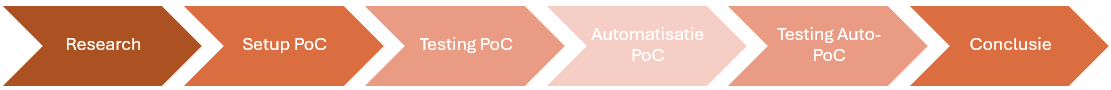
\includegraphics[width=\linewidth]{../graphics/Planning.png}
  \caption{Planning van de methodologie}
  \label{fig:Planning}
\end{figure}

\begin{enumerate}
  \item Research / Voorbereiding
  \item In dienst stellen / Setup
  \item Gebruik en testen
  \item Realisatiefactor bepaling
  \item Conclusie
\end{enumerate}

\section{\IfLanguageName{dutch}{Research / Voorbereidingsfase}{Research / Preparationphase}}%
\label{sec:prep}%
De eerste vraag die moet gesteld worden is: \textit{''Hoe kunnen technologieën worden ingezet om de communicatie aan te pakken in de gezondheidszorg?''}.\\ 

Hiermee wordt de onderzoeksfase gestart. De eerste stap van de onderzoeksfase is het in kaart brengen van het huidige DECT-systeem. Dit zal bekeken worden vanuit een algemeen overzicht. Het doel is om de werking en kenmerken van het DECT-systeem in kaart te brengen .\\
Vervolgens wordt er een opvolgvraag gesteld: \textit{''Wat is het huidige systeem (met \hyphenation{rand-apparatuur}randapparatuur) en wat zijn de nadelen hiervan?''} Hiermee wordt er diepgaand onderzoek gedaan naar het huidige systeem en zijn nadelen. Deze nadelen worden verzameld om achteraf deze te vergelijken het het alternatief.\\ Omdat deze bachelorproef in samenwerking is met 360° Zorglab, zal er onderzocht moeten worden \textit{''Hoe kan een zorgsimulatie worden gesimuleerd?''}. Als dit gekend is kan er een stappenplan worden opgesteld om het alternatief te kunnen testen in zo'n simulatie.
Nadat deze vragen te hebben beantwoord, is het probleem volledig in kaart gebracht.\\

% \item \textit{Welke pogingen zijn al ondernomen om het DECT-systeem als standaard te vervangen?}
% \item \textit{Wat zijn de minimum vereisten voor technologieën, om als alternatief te kunnen \\worden beschouwd?}
% \item \textit{Welke andere communicatie mogelijkheden zijn er die voldoen aan de minimum vereisten?}
% \item \textit{Welke mogelijke data-integratie mogelijkheden hebben de alternatieven?}


Zodra het probleem volledig is gekend, kan men aan de oplossing beginnen. Zo is het belangrijk om te weten: \textit{''Welke pogingen zijn al ondernomen om het DECT-systeem als standaard te vervangen?''} Dit kan inzicht geven in de mogelijke oplossingen. Verder kan men leren uit de tekortkomingenvan vorige pogingen. In combinatie met de vorige pogingen voor een standaardverandering is het noodzakelijk om testbare minimumvereisen te hebben of met andere woorden \textit{''Wat zijn de minimum vereisten voor technologieën, om als alternatief te kunnen worden beschouwd?''}. 
Eenmaal de minimum vereisten gekend zijn kunnen de opgelijste alternatieven onderworpen worden aan deze eisen. Als tussenstap in deze controle wordt elk alternatief ook getoetst op: \textit{''Welke mogelijke data-integratie mogelijkheden hebben de alternatieven?''}. Op deze manier is er een duidelijk antwoord op mogelijke verdere stappen na de bachelorproef voor automatisatie van foutanalyse of foutieve alarmen, met als doel de alarmmoeheid te verminderen en een betere zorg te kunnen bieden aan de patiënt.


% Deze vraag kan enkel beantwoord worden na een kort onderzoek in de verschillende frameworks, architecturen. Als besluit van dit onderzoek zal er een vergelijkende studie zijn. Hieruit wordt het best passende framework gekozen.
% Als vervolg op de keuze van het framework zullen de technische specificaties worden vastgelegd en opgelijst. Dit is een noodzakelijke stap om in de conclusie op het einde een duidelijk beeld te kunnen krijgen van mogelijke upsizing.\\
% De volgende deelvraag is: \textit{''Hoe kan een 5G-netwerk een oplossing bieden?''}.\\ Met deze vraag wordt er dieper onderzoek gedaan naar de huidige 5G-systemen/-frameworks. De laatste deelvraag van de research-/voorbereidingsfase is: \textit{''Hoe moet het 5G-netwerk eruitzien, rekening houdend met framework en scaling?''}\\ Hoewel dit de laatste stap is in de voorbereidende fase, is deze cruciaal voor alle verdere fases. Hier wordt alle informatie vergaard in de researchfase en in een netwerkschema/-topologie verwerkt. Dit zal als leidraad worden gebruikt in het verdere verloop van de bachelorproef.

\section{\IfLanguageName{dutch}{In dienst stellen / Setup-fase}{Setupphase}}%
\label{sec:setup}%
Deze fase bestaat uit het omzetten van de verworven theorie naar een proof-of-concept (PoC). Deze bachelorproef zal bestaan uit 2 PoC's. De eerste zal een simulatie zijn die lokaal op de pc werkt. Het tweede deel is een praktische realisatie, met de artikelen opgelijst in de technische specificaties.

\subsection{\IfLanguageName{dutch}{POC 1: Lokale testomgeving}{poc1}}%
\label{sec:poc1}%
De testomgeving wordt opgesteld op de laptop van de student. Dit zal gebruikmaken van de volgende tools:

\begin{itemize}
    \item Vagrant
    \item Ansible
    \item VirtualBox
\end{itemize}

Zie hoofdstuk \ref{ch:poc1} voor een uitgebreide uitleg van de PoC 1.
\subsection{\IfLanguageName{dutch}{POC2: Praktische realisatie}{poc2}}%
\label{sec:poc2}%

Voor de praktische realisatie wordt er gebruikgemaakt van materiaal aangeleverd door Citymesh en 360° Zorglab. Dit materiaal zal in het zorglab blijven als een vaste opstelling. De noodzakelijke hardware wordt opgesplitst in categorieën:

\begin{itemize}
    \item Software Defined Radio (SDR)
    \item Antenna
    \item Simkaart(en)
    \item Mobiel toestel (5G-compatibel)
    \item Kleine server
\end{itemize}

Deze lijst zal meegroeien met het project.
Zie hoofdstuk \ref{ch:poc2} voor een uitgebreide uitleg van de PoC 2.

\section{\IfLanguageName{dutch}{Gebruik en Testfase}{Usage}}
\label{sec:use}
Het doel van deze fase is het gebruiken en testen van de opstelling. Dit is voor optimalisatie, maar ook voor aftoetsing of de minimumvereisten ook in de praktijk zijn bereikt. De gebruik- en testfase verloopt net zoals de setupfase in twee delen. Het eerste deel is het opstellen van een eenduidig en gedetailleerd testplan. Dit gebeurt voor elke PoC. Hierna volgt de uitvoering van deze testplannen op hun respectievelijke PoC. Het is belangrijk dat tijdens de testfase verschillende activiteiten correct worden uitgevoerd. Zo is het noodzakelijk om gedetailleerde notities te hebben in geval van problemen. Een tweede factor die hier nauw bij samenhangt, is de reproduceerbaarheid van de fout of het probleem. Vervolgens zijn de duur en intensiteit van de test belangrijk. Daarom worden de testplannen meerdere malen doorlopen met een vergrotende tijdsduur en belasting- of gebruikintensiteit. Dit alles wordt ook opgenomen in een testverslag dat in de conclusiefase wordt verwerkt. In dit verslag wordt er ook een antwoord geformuleerd op de vraag: \textit{''Hoe kan de proof of concept voor de simulatie worden aangepast om in realiteit te kunnen gebruiken?''}. Dit zal een onderdeel zijn van de conclusie van het testverslag. Als laatste stap wordt een antwoord geformuleerd op de vraag: \textit{''Welke eigenschappen van het alternatief hebben een vermindering in alarmmoeheid als gevolg?''}.

\section{\IfLanguageName{dutch}{Realisatiefactor bepaling}{realisation}}
\label{sec:realisation}
Deze fase is er om een antwoord te bieden op de vraag: \textit{''Vanaf wanneer is het haalbaar om te implementeren op economisch vlak?''}. Deze vraag komt vanuit Citymesh. Als antwoord hierop wordt er gekeken naar de gradatie van het netwerk en de voordelen ten opzichte van de kosten. Deze afweging wordt zowel gemaakt voor kleine als grote ziekenhuizen. Deze afweging wordt dan gebundeld om het kantelpunt te achterhalen. \\ Voor deze bepaling wordt er gebruikgemaakt van zowel installatiekost als onderhoudskosten, maar ook van de voordelen die nieuwere systemen hebben ten opzichte van het personeel en hun efficiëntie en effectiviteit. 
Zie hoofdstuk \ref{ch:financieel} voor een uitgebreide uitleg van de realisatiefactor of het financieel overzicht.

\section{\IfLanguageName{dutch}{Conclusie}{conclusion}}
\label{sec:conclusion}
In de conclusie is er maar één doel. Dit is de onderzoeksvraag beantwoorden: \textit{''Hoe kunnen technologieën worden ingezet om de communicatie aan te pakken in de gezondheidszorg?''} In deze fase wordt alles uit vorige fases verzameld en verwerkt tot een concreet antwoord en een conclusie op deze vraag. Het eindresultaat zal de bachelorproef zijn. Tenslotte wordt er een korte vergelijking gemaakt van het DECT-systeem met de PoC.
\\\\
Doorheen de hele bachelorproef wordt verwacht dat er een open en directe communicatie is tussen de student en de co-promotoren. Dit is belangrijk omwille van het einddoel van de bachelorproef. Hoewel de onderzoeksvraag een antwoord wil op mogelijke vervanging/integratie, is het de bedoeling dat de tweede PoC in gebruik kan worden genomen door de Hogeschool Gent Departement Gezondheidszorg. Met als doel om een simulatie te kunnen bieden aan de studenten van een vervangoptie van het DECT-systeem, om alarmmoeheid tegen te gaan.



% Voeg hier je eigen hoofdstukken toe die de ``corpus'' van je bachelorproef
% vormen. De structuur en titels hangen af van je eigen onderzoek. Je kan bv.
% elke fase in je onderzoek in een apart hoofdstuk bespreken.

%\input{...}
%\input{...}
%...

%%=============================================================================
%% Conclusie
%%=============================================================================

\chapter{Conclusie}%
\label{ch:conclusie}

% TODO: Trek een duidelijke conclusie, in de vorm van een antwoord op de
% onderzoeksvra(a)g(en). Wat was jouw bijdrage aan het onderzoeksdomein en
% hoe biedt dit meerwaarde aan het vakgebied/doelgroep? 
% Reflecteer kritisch over het resultaat. In Engelse teksten wordt deze sectie
% ``Discussion'' genoemd. Had je deze uitkomst verwacht? Zijn er zaken die nog
% niet duidelijk zijn?
% Heeft het onderzoek geleid tot nieuwe vragen die uitnodigen tot verder 
%onderzoek?

% Het doel van deze thesis is om een alternatief te bieden voor het verouderde DECT-systeem. Dit door eerst het DECT-systeem in kaart te brengen met zijn voordelen en nadelen, maar ook de gebreken en mogelijke problemen. Als eenmaal de gebreken gekend zijn, kan er gekeken worden om deze op te vangen met een moderner systeem zoals 5G. Er zijn echter verschillende alternatieven. Een zeer aanneembare verwachting is dat er zal worden gekozen voor een 5G privaat netwerk, omwille van zijn eigenschappen en de afweging tussen de voor- en nadelen. Hoewel er geen officiële standaard is voor 5G-netwerken binnen de gezondheidszorg, zal er een zo objectief mogelijke keuze worden gemaakt met een vergelijking tussen alle mogelijkheden. Een disclaimer is wel noodzakelijk, aangezien het hier gaat om een bachelorproef zal er voornamelijk gekeken worden naar open-source projecten, omwille van budgetten. \\\\
% De Proof-of-Concept zal een simulatie zijn van een kleinschalig, privaat 5G-netwerk. Hoewel kleinschalig, zal het ontworpen zijn met het oog op schaalbaarheid. Het is te verwachten dat de 5G-oplossing een efficiëntere en accuratere manier voor communicatie zal zijn ten opzichte van het DECT-systeem. Verder wordt er een daling verwacht in het voorkomen van alarmmoeheid. Dit komt doordat er verschillende alarmsignalen gebundeld zullen worden. Er zal ook de mogelijkheid zijn om afbeeldingen of berichten te kunnen sturen, waardoor de arts de situatie van de patiënt beter kan inschatten.\\\\
% Op de vraag vanuit Citymesh voor een techno-economische studie, wordt verwacht dat de kost voor het installeren en uitrollen van het private 5G-netwerk hoog zal zijn in vergelijking met het huidige DECT-systeem. Er zal een afweging moeten worden gemaakt ten opzichte van de kost en de mogelijke winst op lange termijn door welzijn van personeel en daling van incidenten, die te wijten zijn aan alarmmoeheid.\\\\
% De volgende stap na deze bachelorproef is de mogelijke integratie van het systeem in de opleidingen binnen het departement Gezondheidszorg van HOGENT, om de studenten een alternatief te kunnen aanbieden ten opzichte van het DECT-systeem.

In dit onderzoek is gezocht naar een antwoord op de vraag: \textit{''Hoe kan de informatie-uitwisseling tussen artsen en verplegend personeel in ziekenhuizen verbeterd worden door het inzetten van nieuwe technologieën ?''}. Hiervoor is er zowel onderzoek uitgevoerd naar een mogelijke andere technologie als een \gls{poc} opgesteld, waarin een privaat 5G netwerk is gesimuleerd en getest. \\

Uit het onderzoek blijkt dat het \gls{dect}-systeem een  hoge betrouwbaarheid, lage energieconsumptie en een eigen frequentieband met 120 duplex radio kanalen. Echter het is verouderd,  beperkte capaciteit verkeer en slechte integratie. \\

Na het formuleren van de minimumvereisten aan de hand van de MoSCoW methode, zijn volgende eigenschappen noodzakelijk om over een acceptabele vervanging te spreken: Wetgeving conform, gesloten systeem, stabiel en segregatie mogelijkheden. Wel is het noodzakelijk om in het achterhoofd te houden dat het om een vervanging/upgrade gaat dus technologieën moeten minsten gelijkstaan met het \gls{dect}-systeem.\\
Uit de analyse van verschillende technologieën blijkt dat \gls{voip}, \gls{ule} en private 5G-netwerken voldoen aan deze eisen. Deze alternatieven bieden bovendien betere mogelijkheden voor data integratie.\\
Economische haalbaarheid is sterk afhankelijk van de schaal van de implementatie en of er wordt gebruikgemaakt van een gefaseerd project. Verder is de kost groter dan de infrastructuur alleen. Er moet dus niet alleen rekening worden gehouden met de \gls{capex}, maar ook met de \gls{opex}.\\

De eindconclusie kan dus worden opgesplitst in twee delen: een theoretische en een praktische eindconclusie.\\
Theoretisch is een privaat 5G netwerk het effectiefst en het meest toekomstgericht. Dit omdat de data integratie het hoogste ligt en door gebruik te maken van slicing kan met optimale segregatie hebben van communicatiekanalen, al dan niet met prioriteiten. De praktijk schetst natuurlijk ook een beeld, de hoge kost voor het installeren van zo een netwerk kan verschillende ziekenhuizen. Dit omdat men verder kan werken met de huidige installatie mits wat aanpassingen. Een andere optie is het overschakelen naar \gls{voip}, dit is het alternatief met de minste voorkeur omwille van de security.\\

Vervolgonderzoek wou kunnen kijken naar de omzetting naar praktijk, security implementatie en de mogelijke integratie van het systeem in de opleidingen binnen het departement Gezondheidszorg van HOGENT, om de studenten een alternatief te kunnen aanbieden ten opzichte van het DECT-systeem.



%   \item \textit{Wat zijn de kenmerken van het \gls{dect}-systeem?} ✓
%   \item \textit{Wat is het huidige systeem (met \hyphenation{rand-apparatuur}randapparatuur) en wat zijn de nadelen hiervan?}✓
%   \item \textit{Hoe kan een zorgsituatie worden gesimuleerd?}
%   \item \textit{Welke pogingen zijn al ondernomen om het \gls{dect}-systeem als standaard aan te passen?}✓
%   \item \textit{Wat zijn de minimumvereisten voor technologieën, om als alternatief te kunnen worden beschouwd?}✓
%   \item \textit{Welke andere communicatiemogelijkheden zijn er die voldoen aan de minimumvereisten?}✓
%   \item \textit{Welke mogelijke data integratie mogelijkheden hebben de alternatieven?}✓
%   \item \textit{Vanaf wanneer is het haalbaar om te implementeren op economisch vlak?}✓


%---------- Bijlagen -----------------------------------------------------------

\appendix

\chapter{Onderzoeksvoorstel}

Het onderwerp van deze bachelorproef is gebaseerd op een onderzoeksvoorstel dat vooraf werd beoordeeld door de promotor. Dat voorstel is opgenomen in deze bijlage.

%% TODO: 
%\section*{Samenvatting}

% Kopieer en plak hier de samenvatting (abstract) van je onderzoeksvoorstel.

% Verwijzing naar het bestand met de inhoud van het onderzoeksvoorstel
%---------- Inleiding ---------------------------------------------------------

% TODO: Is dit voorstel gebaseerd op een paper van Research Methods die je
% vorig jaar hebt ingediend? Heb je daarbij eventueel samengewerkt met een
% andere student?
% Zo ja, haal dan de tekst hieronder uit commentaar en pas aan.

%\paragraph{Opmerking}

% Dit voorstel is gebaseerd op het onderzoeksvoorstel dat werd geschreven in het
% kader van het vak Research Methods dat ik (vorig/dit) academiejaar heb
% uitgewerkt (met medesturent VOORNAAM NAAM als mede-auteur).
% 

\section{Inleiding}%
\label{sec:inleiding}

In de zorgindustrie wordt er steeds meer gesproken over 'Alarm moeheid.' Dit is een stijgend probleem. Bij alarm moeheid wordt het gezondheidszorgpersoneel overspoeld met een constante vloed van alarmsignalen. Deze moeheid is grotendeels te wijten aan het huidige systeem dat in ziekenhuizen wordt gebruikt. Dit systeem is ook wel gekend als het DECT-systeem. Dit systeem is een audio-systeem, hier zijn de meeste nadelen aan verbonden. Zoals eerder vermeld zullen de overvloed aan alarmsignalen, onder andere gegenereerd door het DECT-systeem, alarm moeheid veroorzaken. Deze moeheid wordt ook versterkt door het belet-systeem, het systeem dat de alarmknop bij de patient plaatst. De moeheid is echter niet het enige probleem. Verder is er een groter probleem en dat is de menselijke factor aan het systeem. Dit wordt duidelijk met een situatie-schets van het gebruik van het DECT-systeem:

\begin{itemize}
  \item Patient bedient alarm knop
  \item Verplegend personeel wordt verwittigd via BELET-systeem
  \item Verplegend personeel reageert op alarm en bezoekt patient
  \item Patient heeft een situatie die verslechtert en verplegend personeel wil dokter inschakelen
  \item Verplegend personeel legt mondeling het probleem uit aan de dokter
  \item Dokter maakt oordeel
\end{itemize}

Het is de voorlaatste stap waar een probleem optreedt. De dokter steunt volledig op de beschrijving van het verplegend personeel. Dit betekent dus ook dat eenmaal de conversatie beeindigd is, is er geen naslagwerk om terug op te vallen.

Deze bachelorproef thesis zal zich focussen op een alternatief voor het DECT-systeem, aan de hand van 5G en is gericht aan IT-personeel in gezondheidszorginstituten. Het primaire doel is om te onderzoeken of het 5G-netwerk een oplossing kan bieden voor de vervanging/modernisering van het DECT-Systeem. Naast het onderzoek zal er een proof of Concept worden opgesteld.

%---------- Stand van zaken ---------------------------------------------------

\section{Literatuurstudie}%
\label{sec:literatuurstudie}

De huidige stand van zaken kan worden opgesplitst in 4 delen. Het eerste deel een situatie schets van de huidige complete set-up, met al hun voordelen en gebreken. Hierna volgt een uiteenzetting van 5G-frameworks, hier gaat het niet alleen over algemene frameworks en bemerkingen over 5G maar ook al meer specifiek gezondheidszorg frameworks van 5G. Nadien wordt er dieper gekeken naar de connectie tussen gezondhseidszorg en 5G, maar ook hun interconnecties. Deze interconnecties bevatten onder andere monitoring integratie. Tenslotte is er een korte toelichting van de cybersecurity verplichtingen in kader van deze bachelorproef.
\\\\
Het DECT-systeem staat voor Digital Enhanced Cordless Telecommunications, dit is een standaard in EU sinds 1993. De meest gebruikte situatie is waar er meerdere gebruikers zijn voor een draadloze communicatie in werkomgevingen. De voornaamste reden voor gebruik van het DECT draadloos systeem is dat het een grote dichtheid van veel gebruikers aankan. Terwijl het in vergelijking met andere mobile communicatie systemen niet werkt buiten de werkomgeving.\autocite{Welinder1997} Na onderzoek van \textcite{Welinder1997} bleek dat de interferentie van het DECT-systeem op medisch gereedschap  was 11 percent. Maar de interferentie valt volledig weg bij een afstand van 0.5m tussen het gereedschap en het DECT toestel.
\\\\
5G is een stap in de evolutie van het mobiele netwerk, opvolger van 4G. Nu het 5G netwerk waar het om draait in deze bachelorproef is het private 5G netwerk. Volgens \textcite{wen2021private} zijn er eigenschappen van private 5G die nauw aansluiten met die van DECT-systemen. De eerste is de hoge device dichtheid, maar bij 5G gaat deze ook nog eens gepaart met hoge throughput. Dit zorgt ervoor dat integratie van externe devices soals sensoren, camera's, etc. Verdergaant op de gelijkenissen in eigenschappen heeft 5G ook voordelen ten opzichte van DECT-systemen volgens \textcite{wen2021private}. Zo Is er een hoge betrouwbaarheid met een lage latency.\\ Verder heeft een privaat netwerk nog het extra voordeel van een aanpasbare voorspelbare Quality of Service (QoS). Daarnaast zijn er verschillende architecturen die men kan implementeren om een privaat 5G netwerk op te zetten. De eerste is een stand-alone deployment, hierbij wordt privaat netwerk opgezet waarbij alle netwerk functies van het netwerk zijn gelimiteerd binnen een logische perimeter bestaande van vooraf gedefinieerde regios. De andere manier is een public netwerk geintegreerd deployment. Deze architectuur kan worden opgesplitst in 3 types, afhankelijk van de gradatie van integratie. Deze 4 types zijn de volgende:

\begin{itemize}
  \item O-RAN (Open Radio Access Network)
  \item Gedeelde RAN (Radio Access Network)
  \item Gedeelde RAN en controle vlak
  \item Hosted bij het Publieke Netwerk
\end{itemize}

\textcite{wen2021private} vermeldt ook dat er naast architectuur ook een keuze moet gemaakt worden voor het spectrum. Hier zijn ook opnieuw 3 keuzes: een Dedicated pirvaat spectrum, een erkend spectrum en een niet-erkend spectrum. 
5G heeft een aantal noodzakelijke technologiën nodig in het netwerk. Een van deze technologiën is network slicing. Hierbij wordt er 'een netwerk in een netwerk' gemaakt door het fysieke netwerk op te splitsen in meerdere logische netwerken. Om aan network slicing te kunnen doen is er een nood aan netwerk virtualisatie. Het silcing zelf kan worden opgedeeld in 3 lagen: Infrastructuur laag, Network slice laag en Onderhouds laag. De levensloop van het slicen van een netwerk verloopt volgens volgende 4 fases \autocite{wen2021private}:

\begin{enumerate}
  \item Voorbereiding
  \item In dienst stellen
  \item Gebruik
  \item Ontmanteling
\end{enumerate}

Het derde luik van de literatuurstudie gaat dieper in op de connecties tussen 5G en gezondheidszorg, en hoe deze worden bereikt aan de hand van bestaande frameworks.
\\\\
In samenspraak met de co-promotor is er geopteerd om cybersecurity niet actief te onderzoeken in deze bachelorproef thesis. Echter het is wel noodzakelijk om te weten dat er verschillende verplichtingen zijn in België en de Europese Unie. Hieronder een kleine verduidelijking als context.
\\
Sinds 27 april 2016 is de verordening 2016/679 van toepassing. Deze start de GDPR (General Data Protection Regulation) in de Europese unie. De verordening 2016/679 vermeldt dat "regels worden vastgelegd betreffende de bescherming van natuurlijke personen in verband met de verwerking van persoonsgegevens en het vrije verkeer van persoonsgegevens. En het beschermt het ook de grondrechten en de fundamentele vrijheden van natuurlijke personen met name hun recht op bescherming van persoonsgegeven."\\ \autocite{gdpr2016} 
\\
Vervolgens is er ook het NIS2, dit is een Belgische wet die bedrijven verplichtingen oplegt op vlak van cybersecurity. "De wet van 26 april 2024 tot vaststelling van een kader voor de cyberbeveiliging van netwerk- en informatiesystemen van algemeen belang voor de openbare veiligheid (de "NIS2-wet") zet de EU-richtlijn 2022/2555 van het Europees Parlement en de Raad van 14 december 2022 (de "NIS2-richtlijn") om." \autocite{Belgium2024}
\\
Tenslotte is er een nieuwer initiatief genaamd EHDS (European Healthcare Data Space). Dit initiatief heeft als algemene doelstelling: "De algemene doelstelling is te waarborgen dat natuurlijke personen in de EU in de praktijk meer zeggenschap over hun elektronische gezondheidsgegevens hebben." \autocite{EHDS2022}

% Voor literatuurverwijzingen zijn er twee belangrijke commando's:
% \autocite{KEY} => (Auteur, jaartal) Gebruik dit als de naam van de auteur
%   geen onderdeel is van de zin.
% \textcite{KEY} => Auteur (jaartal)  Gebruik dit als de auteursnaam wel een
%   functie heeft in de zin (bv. ``Uit onderzoek door Doll & Hill (1954) bleek
%   ...'')

%---------- Methodologie ------------------------------------------------------
\section{Methodologie}%
\label{sec:methodologie}

Alvorens de methodologie volledig wordt besproken is er een belangrijke disclaimer noodzakelijk te vermelden.
In samenspraak met de co-promotoris er geopteerd om cybersecurity niet actief te onderzoeken in deze bachelorproef thesis. Echter het is wel noodzakelijkom te weten dat er verschillende verplichtingen zijn in Belgie en de Europese Unie. In de literatuur studie is er wel een kort naslagwerk van de verplichtingen ten opzichte van cybersecurity.
\\\\
Hier beschrijf je hoe je van plan bent het onderzoek te voeren. Welke onderzoekstechniek ga je toepassen om elk van je onderzoeksvragen te beantwoorden? Gebruik je hiervoor literatuurstudie, interviews met belanghebbenden (bv.~voor requirements-analyse), experimenten, simulaties, vergelijkende studie, risico-analyse, PoC, \ldots?

Valt je onderwerp onder één van de typische soorten bachelorproeven die besproken zijn in de lessen Research Methods (bv.\ vergelijkende studie of risico-analyse)? Zorg er dan ook voor dat we duidelijk de verschillende stappen terug vinden die we verwachten in dit soort onderzoek!

Vermijd onderzoekstechnieken die geen objectieve, meetbare resultaten kunnen opleveren. Enquêtes, bijvoorbeeld, zijn voor een bachelorproef informatica meestal \textbf{niet geschikt}. De antwoorden zijn eerder meningen dan feiten en in de praktijk blijkt het ook bijzonder moeilijk om voldoende respondenten te vinden. Studenten die een enquête willen voeren, hebben meestal ook geen goede definitie van de populatie, waardoor ook niet kan aangetoond worden dat eventuele resultaten representatief zijn.

Uit dit onderdeel moet duidelijk naar voor komen dat je bachelorproef ook technisch voldoen\-de diepgang zal bevatten. Het zou niet kloppen als een bachelorproef informatica ook door bv.\ een student marketing zou kunnen uitgevoerd worden.

Je beschrijft ook al welke tools (hardware, software, diensten, \ldots) je denkt hiervoor te gebruiken of te ontwikkelen.

Probeer ook een tijdschatting te maken. Hoe lang zal je met elke fase van je onderzoek bezig zijn en wat zijn de concrete \emph{deliverables} in elke fase?

%---------- Verwachte resultaten ----------------------------------------------
\section{Verwacht resultaat, conclusie}%
\label{sec:verwachte_resultaten}

Hier beschrijf je welke resultaten je verwacht. Als je metingen en simulaties uitvoert, kan je hier al mock-ups maken van de grafieken samen met de verwachte conclusies. Benoem zeker al je assen en de onderdelen van de grafiek die je gaat gebruiken. Dit zorgt ervoor dat je concreet weet welk soort data je moet verzamelen en hoe je die moet meten.

Wat heeft de doelgroep van je onderzoek aan het resultaat? Op welke manier zorgt jouw bachelorproef voor een meerwaarde?

Hier beschrijf je wat je verwacht uit je onderzoek, met de motivatie waarom. Het is \textbf{niet} erg indien uit je onderzoek andere resultaten en conclusies vloeien dan dat je hier beschrijft: het is dan juist interessant om te onderzoeken waarom jouw hypothesen niet overeenkomen met de resultaten.



%%---------- Andere bijlagen --------------------------------------------------
% TODO: Voeg hier eventuele andere bijlagen toe. Bv. als je deze BP voor de
% tweede keer indient, een overzicht van de verbeteringen t.o.v. het origineel.
%\input{...}

%%---------- Backmatter, referentielijst ---------------------------------------

\backmatter{}

\setlength\bibitemsep{2pt} %% Add Some space between the bibliograpy entries
\printbibliography[heading=bibintoc]

\end{document}
